\documentclass[10pt,a4paper]{amsart}
\usepackage{amsmath,amssymb,amsthm,graphicx}
\usepackage{hyperref}
\usepackage{amssymb}
\numberwithin{equation}{section}

\newtheorem{Theorem}{Theorem}[section]
\newtheorem{Corollary}[Theorem]{Corollary}
\newtheorem{Lemma}[Theorem]{Lemma}
\newtheorem{Proposition}[Theorem]{Proposition}
 { \theoremstyle{definition}
\newtheorem{Definition}[Theorem]{Definition}
\newtheorem{Note}[Theorem]{Note}
\newtheorem{Example}[Theorem]{Example}
\newtheorem{Remark}[Theorem]{Remark} }


\DeclareMathOperator{\Id}{Id}
\DeclareMathOperator{\Span}{Span}
\DeclareMathOperator{\Ann}{Ann}
\DeclareMathOperator{\End}{End}
\DeclareMathOperator{\Hom}{Hom}
\DeclareMathOperator{\Aut}{Aut}

\usepackage{enumitem}
\usepackage{mathrsfs}
% \iffalse meta-comment
%
% File: romanbar.dtx
% Version: 2025-01-28 v1.0g
% Info: Roman numbers with bars
%
% Copyright (C) 2011 - 2025 by
%    H.-Martin Münch <Martin dot Muench at Uni-Bonn dot de>
%
% The original code for the bars was written by Prof. Enrico Gregorio
% (https://profs.sci.univr.it/~gregorio/), and published at
% https://tex.stackexchange.com/a/24084
% I (H.-Martin Münch) submitted this package to CTAN
% (after diverse updates of the code and writing a documentation).
%
% This work may be distributed and/or modified under the
% conditions of the LaTeX Project Public License, either
% version 1.3c of this license or (at your option) any later
% version. This version of this license is in
%    https://www.latex-project.org/lppl/lppl-1-3c.txt
% and the latest version of this license is in
%    https://www.latex-project.org/lppl.txt
% and version 1.3c or later is part of all distributions of
% LaTeX version 2005-12-01 or later.
%
% This work has the LPPL maintenance status "maintained".
%
% The Current Maintainer of this work is H.-Martin Münch.
%
% This work consists of the main source file romanbar.dtx,
% the README, and the derived files
% CTAN romanbar1.0g (H.-Martin Muench), LPPL, embedded macro code.
\makeatletter

%    \end{macrocode}
%
%    \begin{macrocode}
%    \end{macrocode}
%
% A short description of the \xpackage{romanbar} package:
%
%    \begin{macrocode}
%% Allows to write Roman numbers (or any other text) with bars
%% and to convert Arabic numbers into Roman ones.
%    \end{macrocode}
%
% There are no options to be processed.
%
%    \begin{macrocode}

\RequirePackage{trimclip}[2020/08/19]% v1.2

\newcounter{romanbarcount}
\newdimen\romanbardimH
\newdimen\romanbardimD
\newdimen\romanbardimW

%    \end{macrocode}
%    \begin{macro}{\gobbleminus}
%
% A command to gobble a possible minus sign is needed and
% |\gobbleminus| from \url{https://texfaq.org/FAQ-isitanum}
% is used.
%
%    \begin{macrocode}
\def\gobbleminus#1{\ifx-#1\else#1\fi}
%% from https://texfaq.org/FAQ-isitanum

%    \end{macrocode}
%    \end{macro}
%    \begin{macro}{\ifnumeric}
%
% We want to test whether the argument passed to |\Romanbar| is numeric
% and therefore define |\ifnumeric{test}{true}{false}|,
% where |test| is to be analysed, |true| is the code to be executed,
% if |test| is numeric, and |false| is the code to be executed,
% if |test| is not numeric. This is done similar to
% \url{https://tex.stackexchange.com/a/17119}.
%
%    \begin{macrocode}
\newcommand{\ifnumeric}[3]{%
%% similar to https://tex.stackexchange.com/a/17119
\sbox\z@{\c@romanbarcount=0\gobbleminus#1\relax}%
\ifdim\wd0>\z@\relax#3% is not numeric
\else#2% is numeric
\fi%
}

%    \end{macrocode}
%    \end{macro}
%    \begin{macro}{\r@iseL}
%
% We define |\r@iseL| to raise any L~(50), otherwise a good deal
% of the horizontal part of the letter would be swallowed by the lower bar
% under the \textquotedblleft number\textquotedblright .
%
%    \begin{macrocode}
\def\r@iseL#1{\ifx @#1% then terminate
\else%
\if L#1\raisebox{0.05ex}{\begin{clipbox}{0pt 0pt 0pt 0.05ex}L\end{clipbox}}%
\else #1\fi%
\expandafter\r@iseL%
\fi%
}

%    \end{macrocode}
%    \end{macro}
%    \begin{macro}{\Romanbar}
%
% We define the |\Romanbar| command.
%
%    \begin{macrocode}
\DeclareRobustCommand{\Romanbar}[1]{%
\ifnumeric{#1}{% is numeric
%    \end{macrocode}
%
% If its parameter is numeric, the temporary counter |romanbarcount| is set to the value.
%
%    \begin{macrocode}
\setcounter{romanbarcount}{#1}%
%    \end{macrocode}
%
% Regularly there are no non-positive Roman numbers, therefore we do some trick
% similar to |\XRoman| from the \url{https://ctan.org/pkg/pageslts} package.
%
%    \begin{macrocode}
%% similar to \XRoman from the https://ctan.org/pkg/pageslts package
\ifnum\theromanbarcount<1%
  \ifnum #1>0\relax%
    \Roman@bar{\Roman{#1}}%
  \else%
    \ifnum #1<0\relax%
      -\Roman@bar{\expandafter\@slowromancap\romannumeral\number-#1@}%
    \else%
      \Roman@bar{0}%
    \fi%
  \fi%
\else\Roman@bar{\@Roman\c@romanbarcount}%
\fi%
}{% is not numeric
\Roman@bar{#1}%
}%
}

%    \end{macrocode}
%    \end{macro}
%    \begin{macro}{\Roman@bar}
%
% Whether it is numeric or not, in the end |\Roman@bar| is applied to it.
%
%    \begin{macrocode}
\DeclareRobustCommand{\Roman@bar}[1]{% #1 is in Roman, i.e. MMXXIII
%% (or any other text, "Caesar" would work, too);
%% similar to code of  by Prof. Enrico Gregorio (egreg) at
%% https://tex.stackexchange.com/a/24084
\@bsphack%
\edef\romanbartmp{#1}%
%% height:
\sbox0{\textsf{\romanbartmp}}%
%% top line:
%% + top of top line:
\setlength{\romanbardimH}{\dimexpr\ht0+0.05ex\relax}%
%% + bottom of top line:
\setlength{\romanbardimD}{\dimexpr-\ht0+0.05ex\relax}%
%% width:
\sbox0{\textsf{\expandafter\r@iseL\romanbartmp @}}%
\setlength{\romanbardimW}{\dimexpr\wd0+1pt\relax}%
\@esphack%
\makebox[\romanbardimW]{%
\rlap{\vrule width\romanbardimW height\romanbardimH depth\romanbardimD}% top line
\rlap{\vrule width\romanbardimW height 0.06ex       depth 0.03ex}%    bottom line
\kern0.5pt\textsf{\expandafter\r@iseL\romanbartmp @}\kern0.5pt}%
}

%    \end{macrocode}
%    \end{macro}
%    \begin{macro}{\romannum}
%
% While it is not needed for the bars, it is sometimes asked for a command
% to convert an Arabic number into a Roman one. |\roman{...}| can only be applied
% to a counter, i.\,e.~|\roman{25}| does not work, but
%\begin{verbatim}
%\newcounter{examplecounter}
%\setcounter{examplecounter}{25}
%\roman{examplecounter}
%\end{verbatim}
% would be necessary. Further non-negative values would not work.
% |\romannum| accepts any number as argument. (If the argument is no number,
% an error message is given and the argument printed (executed)
% without applying anything to it.)
%
%    \begin{macrocode}
\DeclareRobustCommand{\romannum}[1]{%
\ifnumeric{#1}{% is numeric
\setcounter{romanbarcount}{#1}%
%% similar to \xroman from the https://ctan.org/pkg/pageslts package
\ifnum\c@romanbarcount<1\relax%
  \ifnum #1>0\relax%
    \roman{#1}%
  \else%
    \ifnum #1<0\relax%
      -\romannumeral\number-#1@%
    \else%
      0%
    \fi%
  \fi%
\else\@roman\c@romanbarcount%
\fi%
}{% is not numeric
\PackageError{romanbar}{%
Argument of \string\romannum\space is not a number}{%
The command \string\romannum\space converts an Arabic number into a %
lower-case Roman one,\MessageBreak%
but the used argument of \string\romannum\space is not an Arabic number %
but\MessageBreak%
`#1`,\MessageBreak%
which will now be printed unchanged.}%
#1%
}%
}

%    \end{macrocode}
%    \end{macro}
%    \begin{macro}{\Romannum}
%
% The same for upper-case Roman numbers, |\Romannum| instead of |\Roman|:
%
%    \begin{macrocode}
\DeclareRobustCommand{\Romannum}[1]{%
\ifnumeric{#1}{% is numeric
\setcounter{romanbarcount}{#1}%
%% similar to \XRoman from the http://ctan.org/pkg/pageslts package
\ifnum\c@romanbarcount<1\relax%
  \ifnum #1>0\relax%
    \Roman{#1}%
  \else%
    \ifnum #1<0\relax%
      -\expandafter\@slowromancap\romannumeral\number-#1@%
    \else%
      0%
    \fi%
  \fi%
\else\@Roman\c@romanbarcount%
\fi%
}{% is not numeric
\PackageError{romanbar}{%
Argument of \string\Romannum\space is not a number}{%
The command \string\Romannum\space converts an Arabic number into an %
upper-case Roman one,\MessageBreak%
but the used argument of \string\Romannum\space is not an Arabic number %
but\MessageBreak%
`#1`.}%
#1%
}%
}

%    \end{macrocode}
%    \end{macro}
%    \begin{macrocode}
\makeatother
\newcommand{\II}{\mathrm{I\hspace{-.1em}I}}

\allowdisplaybreaks[4]
\pdfstringdefDisableCommands{\def\boldsymbol#1{#1}}
\title{Generalized Weyl algebra realization of the symplectic differential reduction algebra}
\author{Jonas T. Hartwig, Dwight Anderson Williams II}
\date{doi:10.3842/SIGMA.2025.001; CC BY 4.0}
\begin{document}
\maketitle
\noindent\textit{Allowed standard prerequisites (editorial).}\begin{itemize}
\item Research prerequisites named in the original article. Full original bibliography retained; all source-local definitions and supporting arguments retained.
\end{itemize}\medskip
\section{Introduction}\label{sec:Intro}

\subsection{Background}\label{subsec:Background}
Mickelsson addressed the problem of reducing representations of Lie algebras over a subalgebra with the introduction of step algebras \cite{mickelssonStepAlgebrasSemisimple1973}, which are now known as Mickelsson algebras. These algebras are part of a broader family, collectively called \emph{reduction algebras} \cite{khoroshkinDiagonalReductionAlgebras2010}.
Specific applications and developments relying on reduction algebras are found in the decomposition of tensor product modules (via actions of diagonal reduction algebras) \cite{hartwigDiagonalReductionAlgebra2022c,khoroshkinDiagonalReductionAlgebras2010}, higher-order Fischer decompositions in harmonic analysis \cite{debieHarmonicTransvectorAlgebra2017}, conformal field theory \cite{conleyBoundedLengthRepresentations2001,conleyConformalSymbolsAction2009}, and the construction of wave functions \cite{asherovaProjectionOperatorsSimple1973} in the realm of theoretical particle and nuclear physics, as examples. The last paper formalized extremal projectors, and Zhelobenko \cite{zhelobenkoExtremalProjectorsGeneralized1989} is credited with realizing the importance of extremal projectors in a scheme to determine generators and relations of localized reduction algebras. See \cite{zhelobenkoPrincipalStructuresMethods2006} for an overview of the construction of generalized Mickelsson algebras.


The crucial observation is that reduction algebras associated to a reductive Lie algebra $\mathfrak{g} = \mathfrak{g}_{-} \oplus \mathfrak{h} \oplus \mathfrak{g}_{+}$ generally arise from a triple of data, that is, a Lie algebra homomorphism $\Xi\colon \mathfrak{g} \rightarrow A$ from $\mathfrak{g}$ to an associative algebra $A$ or the resulting algebra map (perhaps also called $\Xi$) from the universal enveloping algebra $U(\mathfrak{g})$ of $\mathfrak{g}$ to $A$. We set $I$ to be the left ideal in $A$ generated by the positive nilpotent subalgebra $\mathfrak{g}_{+} \subset \mathfrak{g}$ via the $\Xi$-induced action of $\mathfrak{g}$ on $A$. Then the reduction algebra $Z = Z(A,\mathfrak{g},\Xi)$, up to a choice of localization, is the subquotient $N/I$, where the normalizer $N$ is the largest subalgebra of $A$ containing $I$ as a two-sided ideal. A common case occurs when $\Xi$ is an embedding of $\mathfrak{g}$ into the universal enveloping algebra $U(\mathfrak{t})$ of a Lie algebra $\mathfrak{t} \supset \mathfrak{g}$ containing $\mathfrak{g}$, and we write simply $Z = Z(\mathfrak{t},\mathfrak{g})$. The same abbreviation of the map occurs in the super analogue or whenever the Lie (super)algebra homomorphism is understood. There is also a $q$-analog of this construction using Drinfeld--Jimbo quantum groups.

We now emphasize two points. The first is that reduction algebras are associative algebras with their own lanes of study. There are a great number of results on reduction algebras with many summarized at the end of Tolstoy's commemorative paper \cite{tolstoy2005fortieth}. Khoroshkin and Ogievetsky furthered results by giving a complete presentation of the diagonal reduction algebra \cite{khoroshkinDiagonalReductionAlgebras2010} of type $A$ of any rank.
With motivation drawn from the second author's work \cite{williamsii2020BasesInfinitedimensionalRepresentations,williamsii2024actionosp12npolytensor} on finding explicit bases of tensor product representations of the orthosymplectic Lie superalgebras~$\mathfrak{osp}(1|2n)$, we gave a complete presentation \cite[Section~3.5]{hartwigDiagonalReductionAlgebra2022c} of the diagonal reduction superalgebra $Z(\mathfrak{osp}(1|2) \times \mathfrak{osp}(1|2), \mathfrak{osp}(1|2))$, the first recorded diagonal reduction algebra associated to a classical \cite{kacClassificationSimpleLie1979} Lie superalgebra. In the sequel \cite{hartwigGhostCenterRepresentations2023}, we classified finite-dimensional and certain infinite-dimensional representations of $Z(\mathfrak{osp}(1|2) \times \mathfrak{osp}(1|2), \mathfrak{osp}(1|2))$.

The second matter is that homomorphisms to the $n$-th Weyl algebra $A_{n}$ (see the use of \emph{canonical realizations} in \cite[Definition 1]{havlicekCanonicalRealizationsLie1975}) yield examples of reduction algebras important to quantum deformations and noncommutative geometry. A particular example is the ring $\mathcal{D}_{\mathbf{h}}(n,N)$ of $\mathbf{h}$-deformed differential operators \cite{herlemontDifferentialCalculusMathbf2017}. It is the reduction algebra defined from the diagonal map sending $\mathfrak{gl}(n)$ to (a localization of) the tensor product $U(\mathfrak{gl}(n)) \otimes A_{nN}$; the first factor relies on the definition of $U(\mathfrak{gl}(n))$, and the second factor uses $N$-copies of an oscillator realization of~$\mathfrak{gl}(n)$.

In this paper, we combine the two points of emphasis above: We initiate the study of the symplectic analogue of $\mathcal{D}_{\mathbf{h}}(2,1)$ by extending a classical oscillator realization of the rank two symplectic Lie algebra $\mathfrak{sp}(4)$ within $A_{2}$ such that the codomain algebra $A$ is the tensor product~${A_2\otimes U(\mathfrak{sp}(4))}$. We localize $A$ to an algebra $\mathscr{A}$ in order to satisfy certain conditions allowing for the use of the $\mathfrak{sp}(4)$ extremal projector.
After sorting out preliminaries in Section \ref{sec:PreliminariesRedAlg}, we use the extremal projector to present a complete set of generators and relations of the \emph{symplectic differential reduction algebra} $D(\mathfrak{sp}(4)) \cong Z(\mathscr{A},\mathfrak{sp}(4))$ in Section \ref{sec:sp4reduction}. Furthermore, we remark that there is a homomorphism from the diagonal reduction algebra of $\mathfrak{sp}(4)$ to $D(\mathfrak{sp}(4))$, and therefore our presentation of the latter should be helpful in finding a presentation of the former.
Lastly, we show in Section \ref{sec:GWA} that after a change of generators, $D(\mathfrak{sp}(4))$ is manifestly a generalized Weyl algebra (GWA) of a new and interesting type. In particular, the irreducible weight modules over $D(\mathfrak{sp}(4))$ can now be classified by understanding orbits and breaks in the maximal spectrum. See \cite{bavula1992generalized,hartwigNoncommutativeFiberProducts2018,mazorchukAssociativeAlgebrasRelated2003}.

\section{Preliminaries}\label{sec:PreliminariesRedAlg}
The base field is $\mathbb{C}$ except when specified otherwise.

\subsection{Oscillator realization and Chevalley generators}\label{subsec:Oscillator-Chevalley}

{\bf Weyl algebras.}
Let $A_{n}$ denote the $n$-th Weyl algebra. Thus, $A_{n}$ is the complex associative algebra with generators~$x_{i}$, $\partial_{i} = \frac{\partial}{\partial x_{i}}$, for $i=1,2,\dots,n$, and relations
\begin{align}\label{eq:weylrels}
	x_ix_j-x_ jx_i =0,\qquad
	\partial_i\partial_j-\partial_j\partial_i =0,\qquad
	\partial_ix_j-x_j\partial_i =\delta_{ij},
\end{align}
where $\delta_{ij}$ is the Kronecker delta. The Weyl algebra $A_{n}$ carries an involutive anti-automor\-phism\footnote{That is, $\vartheta$ is $\mathbb{C}$-linear, $\vartheta(ab)=\vartheta(b)\vartheta(a)$, and $\vartheta^2=\Id_{A_n}$.}~$\vartheta$, called the symplectic Fourier transform, uniquely determined by
\begin{equation}\label{eq:vartheta}
	\vartheta(x_{i})=\partial_{i}.
\end{equation}

{\bf The rank two symplectic Lie algebra.}
Let $\mathfrak{g}=\mathfrak{sp}(4)$ be the $10$-dimensional complex simple Lie algebra of Cartan type $C_2$. It consists of all $4\times 4$ matrices of the form $\left[\begin{smallmatrix}A&B\\C&D\end{smallmatrix}\right]$ where~$B$ and $C$ are symmetric $2\times 2$ matrices, $A$ is any $2\times 2$ matrix, and $D=-A^{\mathsf{T}}$.
The oscillator realization of $\mathfrak{sp}(4)$ is a canonical algebra homomorphism $\omega\colon U(\mathfrak{sp}(4))\to A_2$; see, for example, \cite[Section~4.6]{dixmierEnvelopingAlgebras1996} or \cite{havlicekCanonicalRealizationsLie1976}.
The image of $\mathfrak{sp}(4)$ is $\Span_\mathbb{C}\{uv+vu\mid u,v\in\{x_1,x_2,\partial_1,\partial_2\}\}$.
Since $\mathfrak{sp}(4)$ is simple, we may thus identify $\mathfrak{sp}(4)$ with the $10$-dimensional Lie subalgebra of $A_{2}$ spanned by $\{a_{ij}, b_{ij}, c_{ij} \mid i = 1,2\}$, where
\begin{equation}\label{eq:sp4-oscillator}
	a_{ij} = \frac{1}{2}(x_i\partial_j+\partial_jx_i)=x_i\partial_j+\frac{1}{2}\delta_{ij},\qquad
	b_{ij} = b_{ji} = x_ix_j,\qquad
	c_{ij} = c_{ji} = \partial_i\partial_j.
\end{equation}

Note that $\vartheta$ from \eqref{eq:vartheta} preserves the subspace $\mathfrak{sp}(4)\subset A_2$. We identify $\vartheta|_{\mathfrak{sp}(4)}$ with the involutive Lie algebra anti-automorphism $\tau$ given by
$\tau(a_{ij})=a_{ji}$, $ \tau(b_{ij})=c_{ij}$.

After this identification, the subspace $\mathfrak{h}= \mathbb{C} a_{11} \oplus \mathbb{C} a_{22}$ is a Cartan subalgebra of $\mathfrak{sp}(4)$. We use standard notation for the $8$ roots of $\mathfrak{sp}(4)$, which are
$\pm 2\epsilon_{1}$, $\thinspace \pm 2\epsilon_{2}$, $\thinspace \pm(\epsilon_{1}-\epsilon_{2})$, $\thinspace \pm(\epsilon_{1}+\epsilon_{2})$,
denoting the simple roots by $\alpha = \epsilon_1-\epsilon_2$, $\beta = 2\epsilon_2$. The set of positive roots is $\Phi_+=\{\beta, \beta+\alpha, \beta+2\alpha, \alpha\}$.
There are exactly two convex orderings \cite{itoClassificationConvexOrders2001} of the positive roots
\[%\label{eq:sp4-convex-orderings}
	\beta<\beta+\alpha<\beta+2\alpha<\alpha,\qquad
	\alpha<\beta+2\alpha<\beta+\alpha<\beta.
\]
The corresponding root system is shown in Figure \ref{fig:C2}.

\begin{figure}[ht]
	\centering
	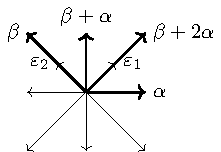
\includegraphics{C2-root-system.pdf}
	\caption{Root system of type $C_2$. Thick lines indicate a choice of positive roots.}
\label{fig:C2}
\end{figure}

Fix positive root vectors, with
${\rm i}=\sqrt{-1}$:
\begin{align*}
	e_{\alpha} = a_{12}, \qquad e_{\beta} = \frac{{\rm i}}{2}b_{22},\qquad
	e_{\beta+\alpha} =[e_{\alpha},e_\beta],\qquad e_{\beta+2\alpha}=\frac{1}{2}[e_\alpha,e_{\beta+\alpha}].
\end{align*}
These provide $\mathfrak{sl}(2)$-triples $(e_{\gamma},f_{\gamma},h'_{\gamma})$, where $f_{\gamma}=\tau(e_{\gamma})$ and $h'_{\gamma}=[e_{\gamma},f_{\gamma}]$:
\begin{gather*}
		\alpha\colon\ (a_{12},\thinspace a_{21},\thinspace a_{11} - a_{22}) = (x_{1}\partial_{2},\thinspace x_{2}\partial_{1},\thinspace x_{1}\partial_{1}-x_{2}\partial_{2}),\\
		\beta\colon\ \left(\frac{\rm i}{2}b_{22},\thinspace \frac{\rm i}{2}c_{22},\thinspace a_{22}\right) = \left(\frac{\rm i}{2}x^{2}_{2}x_{2},\thinspace \frac{\rm i}{2}\partial^{2}_{2},\thinspace x_{2}\partial_{2} + \frac{1}{2}\right),\\
		\beta + \alpha\colon\ ({\rm i} b_{12},\thinspace {\rm i} c_{12},\thinspace a_{11} + a_{22}) = ({\rm i}x_{1}x_{2},\thinspace {\rm i}\partial_{1}\partial_{2},\thinspace x_{1}\partial_{1} + x_{2}\partial_{2} + 1),\\
		\beta + 2\alpha\colon\ \left(\frac{\rm i}{2}b_{11},\thinspace \frac{\rm i}{2}c_{11},\thinspace a_{11}\right) = \left(\frac{\rm i}{2}x_{1}x_{1},\thinspace \frac{\rm i}{2}\partial_{1}\partial_{1},\thinspace x_{1}\partial_{1} + \frac{1}{2}\right).
\end{gather*}
We reserve $h_\gamma$ for the following integer-shifted coroots,
which will simplify computations
\[%\label{eq:shifted-coroots-lowercase}
	h_\alpha = h_\alpha',\qquad h_{\beta+2\alpha}=h_{\beta+2\alpha}'+1,\qquad h_{\beta+\alpha}=h_{\beta+\alpha}'+2,\qquad h_\beta=h_\beta',
\]
where $h'_{\beta+\alpha} = h_{\alpha} + 2h_{\beta}$ and $h'_{\beta+2\alpha} = h_{\alpha} + h_{\beta}$.
The simple coroots satisfy $\alpha(h_{\beta})=-1$, $\beta(h_{\alpha})=-2$.
Also, note that any scalar shift of $h'_{\alpha+\beta}$ yields the total degree derivation on $A_{2}$ in the adjoint representation:
$[x_{1}\partial_{1} + x_{2}\partial_{2} + 1, x_i]=x_i$ and $[x_{1}\partial_{1} + x_{2}\partial_{2} + 1, \partial_i]=-\partial_i$.


{\bf The map $\boldsymbol{\zeta}$.}
Composing the usual comultiplication in $U(\mathfrak{sp}(4))$ with the oscillator representation in the first tensor leg, we obtain an algebra homomorphism
\begin{equation}\label{eq:Homomorphism-sp4toA}
	\zeta\colon\ U(\mathfrak{sp}(4)) \rightarrow A_{2}\otimes U(\mathfrak{sp}(4)),\qquad v\mapsto \omega(v)\otimes 1+1\otimes v.
\end{equation}

We denote the images of the $\mathfrak{sl}(2)$-triples under $\zeta$ by $(E_\gamma,F_\gamma,H'_\gamma)$.
Similarly, put
\[H_\alpha = H_\alpha',\qquad H_{\beta+2\alpha}=H_{\beta+2\alpha}'+1,\qquad H_{\beta+\alpha}=H_{\beta+\alpha}'+2,\qquad H_\beta=H_\beta'.\]

\begin{Remark}
	The tensoring of $A_{2}$ with $U(\mathfrak{sp}(4))$ is useful for the study of tensor product representations in which one tensor factor is an oscillator representation of $\mathfrak{sp}(4)$; however, the authors stress that there is no requirement in general for the codomain algebra to contain~$U(\mathfrak{sp}(4))$ in order to study or apply reduction algebras. We observe that \eqref{eq:sp4-oscillator} does not yield an injective algebra homomorphism from $U(\mathfrak{sp}(4))$ to $A_{2}$ as, amongst many relations, $b_{12}c_{12} - a_{12}a_{21} + a_{11} - \frac{1}{2} = 0$. Yet one can study the associated reduction algebra, a topic we review next.
\end{Remark}

\subsection{Reduction algebras}\label{subsec:ReductionAlgebras}
There is extensive literature \cite{ashtonRmatrixMickelssonAlgebras2015,hartwigGhostCenterRepresentations2023,khoroshkinMickelssonAlgebrasZhelobenko2008,herlemontRingsHdeformedDifferential2017,vandenhomberghNoteMickelssonStep1975,zhelobenkoExtremalProjectorsGeneralized1989,zhelobenkoHypersymmetriesExtremalEquations1997} on reduction algebras and their applications.
We provide a brief overview of constructions/perspectives and related notions for when $\mathfrak{g}$ is a~complex finite-dimensional reductive Lie algebra $\mathfrak{g}=\mathfrak{g}_{-}\oplus\mathfrak{h}\oplus\mathfrak{g}_{+}$ with fixed (maximal) nilpotent subalgebras $\mathfrak{g}_{\pm}$ and Cartan subalgebra $\mathfrak{h}$. See \cite[Section~2]{hartwigDiagonalReductionAlgebra2022c} for details in the super case.

{\bf Subquotient algebra.} Let $A$ be an associative algebra and $\Xi\colon U(\mathfrak{g})\to A$ a map of associative algebras. In particular, the map $\Xi$ makes $A$ into a $U(\mathfrak{g})$-bimodule via multiplication. Let~${I=A\cdot \mathfrak{g}_+}$ (written as $A\mathfrak{g}_+$ from hereon) be the left ideal in $A$ generated by the image of~$\mathfrak{g}_+$ under $\Xi$ composed with the natural inclusion. The reduction algebra $Z = Z(A,\mathfrak{g},\Xi)$ equals~${N_{A}(I)/I}$, where $N_{A}(I)$ is the normalizer of $I$ in $A$. To clarify, the \emph{normalizer} $N_{A}(I)$ of the left ideal $I$ in $A$ is the maximal subalgebra of $A$ with respect to containment of $I$ as a~two-sided ideal. Hence as an $A$-subquotient the reduction algebra $Z$ inherits its product from $A$. Note that normalizers may be termed \emph{idealizers} in general ring theory \cite[specifically Section~2 for historical context]{jacobsonNonCommutativePolynomialsCyclic1934}.

\begin{Remark}
	As mentioned in the introduction, the necessary data is encoded in a Lie algebra map $\Xi\colon \mathfrak{g} \rightarrow A$. Reduction algebras may be expressed as $Z(\mathfrak{t},\mathfrak{g})$ (respectively, $Z(A, \mathfrak{g})$) if the map $\mathfrak{g} \rightarrow U(\mathfrak{t})$ (respectively, $\mathfrak{g} \rightarrow A$) is given in context.
\end{Remark}

{\bf Opposite endomorphism algebra.} As $(\End_{A}(A))^{\mathrm{op}}$ is isomorphic to $A$, one might hope for a natural realization of the $A$-sub\-quo\-tient $Z$ as endomorphisms of an $A$-module.
Indeed, since $n \in N_{A}(I)$ implies $In \subset I$, right multiplication by $N_{A}(I)$ defines a right action on $A/I$ such that $I \subset \Ann_{N_{A}(I)}(A/I)$. It follows that $A/I$ is a right $Z$-module, in fact, an $(A,Z)$-bimodule. Then $\End_{A}(A/I)$ is a left $Z$-module isomorphic to the left $Z$-module $Z$, particularly since endomorphisms of $A/I$ preserve $Z$ and $1+I \in Z$ generates $A/I$ as an $A$-module. Now consider maps $1+I \mapsto n+I$, $n \in N_{A}(I)$, which are precisely the elements of $\End_{A}(A/I)$ by the previous statement. Then opposite composition shows that the reduction algebra $Z$ is isomorphic to $Z_{\text{maps}} = (\End_{A}(A/I))^{\mathrm{op}}$, the opposite algebra of left $A$-module endomorphisms on $A/I$.

{\bf Invariants.}
For a left $A$-module $V$, the subspace of $\mathfrak{g}_{+}$-invariants is $V^{+} = \{{v \in V \mid ev = 0} \allowbreak \text{for all } e\in \mathfrak{g}_{+} \}$.
Then since $N_{A}(I)V^{+} \subset V^{+}$ and $IV^{+} = \{0\}$, there is a natural action on~$V^{+}$ by~$Z$ on the left. Taking the case where $V = A/I$, we have that $Z = (A/I)^{+}$ since ${\mathfrak{g}_{+}(a + I) = \{0 + I\}}$ if and only if $Ia \subset I$, the defining condition for $a \in N_{A}(I)$. We say then that $A/I$ is the universal $\mathfrak{g}_{+}$-highest-weight $A$-module in the sense that given a pair $(W,w)$ of a~left $A$-module $W$ containing a (singular) vector $w$ (such as any $\mathfrak{g}_{+}$-highest-weight vector), there exists a unique $A$-module homomorphism $\Psi_{w}\colon A/I \rightarrow W$ sending $1+I$ to $w$. Evaluation at~${1+I \in (A/I)^{+}}$ determines $\Psi_{w}$ completely; thus, the left $Z$-module $\Hom_{A}(A/I,W)$ and $W^{+}$ are isomorphic
as left $Z$-modules, as in the special case in the previous paragraph.

\begin{Remark}
	Recasting $W^{+}$ as solutions to a system of equations puts $Z$ as a symmetry algebra of the solution space. In particular, reduction algebras are useful in determining solutions to so-called extremal equations \cite{zhelobenkoHypersymmetriesExtremalEquations1997}.
\end{Remark}

{\bf Coinvariants.}
There is a dual construction of reduction algebras based on $\mathfrak{g}_{-}$-coinvariants, the elements of $V_{-} = V/\mathfrak{g}_{-}V$ for a left $A$-module $V$ (taking into account the action of $\mathfrak{g}_{-}$ induced by $\Xi$).
We begin with the quotient space $(A/I)_{-} = (A/I)/\mathfrak{g}_{-}(A/I)$ that comprises the $\mathfrak{g}_{-}$-coinvariants of $A/I$. Note that $A/I$ being a right $Z$-module and $A$ being a $U(\mathfrak{g})$-bimodule implies $(A/I)_{-}$ is a right $Z$-module. By multiple applications of the fundamental theorem of homomorphisms and setting the right ideal $\mathfrak{g}_{-}A$ equal to $J$, we identify $(A/I)_{-}$ with the double coset space $J\reflectbox{$/$}A/I = A/\Romanbar{II}$, where $\Romanbar{II}$ is the sum of abelian groups $I + J$. Explicitly, the mapping sending $(a + I) + \mathfrak{g}_{-}(A/I) \in (A/I)_{-}$ to $a + (I + J) \in a + \Romanbar{II}$ is an isomorphism of vector spaces. Then we have the composition $\nu = \pi\circ\iota\colon Z \rightarrow A/\Romanbar{II}$ of right $Z$-modules from the natural inclusion~${\iota\colon Z\rightarrow A/I}$ and the natural surjection $\pi\colon A/I \rightarrow A/\Romanbar{II}$.

{\bf Extremal projector.} %\label{subsubsec:ExtremalProjector}
The use of $\Romanbar{II}$ for the sum $I+J$ of abelian groups is suggestive as the resulting quotient $A/\Romanbar{II}$ of $\mathfrak{g}_{-}$-coinvariants has the structure of an algebra isomorphic to $Z$ via the extremal projector.
Extremal projectors were introduced in \cite{lowdinAngularMomentumWavefunctions1964} and subsequently studied by Asherova, Smirnov, Tolstoy \cite{asherovaProjectionOperatorsSimple1973}.
Each finite-dimensional reductive Lie algebra $\mathfrak{g}$ over the complex numbers admits a unique extremal projector $P_{A,\mathfrak{g},\Xi} = P_{\mathfrak{g}} = P_{\mathfrak{g}_{+}} = P$ (varying only in expression) that projects the universal $\mathfrak{g}_{+}$-highest-weight $A$-module $A/I$ (more generally, an $A$-module $V$) onto the space of invariants $Z$ (respectively, $V^{+}$) along $J$ (respectively, $\mathfrak{g}_{-}V)$ when the input data $(A,\mathfrak{g},\Xi)$ satisfies sufficient conditions:
\begin{enumerate}[label=(C\arabic*)]\itemsep=0pt
	\item With the adjoint action, the Lie algebra $\mathfrak{g}$ acts reductively on $A$ via $\Xi$. \label{EPconditons:1:adjoint}
	\item The left action of $\mathfrak{g}_{+}$ on $A$ (or on $V$) is locally finite. \label{EPconditons:2:locally-finite}
	\item The image $\Xi(h-n)$ is invertible in $A$ for any coroot $h$, integer $n$ (\emph{coroot condition}). \label{EPconditons:3:coroot-condition}
\end{enumerate}
Using the categorical language of \cite{andreotti1957generalites}, we have $\nu^{-1} = (\pi \circ \iota)^{-1}$ is the $(A,Z)$-bimodule map coming by considering first the astriction of $P$ to $A/\Romanbar{II}$ (descending $P$ to $A/\Romanbar{II}$) before requiring the coastriction of the resulting map to its image, which is equal to $\operatorname{Im}(P) = Z$ (shrinking the codomain to $Z$): \smash{$A/I \xrightarrow{\pi} A/\Romanbar{II} \xrightarrow{\nu^{-1}} Z \xrightarrow{\iota} A/I$}. Then, as noted by Khoroshkin and Ogievetsky, we get the \emph{double coset algebra}:

\begin{Proposition}[{\cite[equation (3.7)]{khoroshkinMickelssonAlgebrasZhelobenko2008}}]\label{thm:double-coset-algebra}
	Under conditions {\rm\ref{EPconditons:1:adjoint}}, {\rm\ref{EPconditons:2:locally-finite}}, and {\rm\ref{EPconditons:3:coroot-condition}},
	there is an associative binary product $\diamond$ $($``diamond product''$)$ on $A/\II$, defined by
	\[\bar{x} \diamond \bar{y} = \pi(xP(y+I)), \qquad \bar{x} = x+ \II,\thinspace \bar{y} = y + \II\thinspace \in A/\emph{\Romanbar{II}},\]
	which yields $\nu^{-1}$ as an isomorphism of associative algebras: $A/\emph{\Romanbar{II}} \cong Z$.
	
	Note: We use $xPy + \II$ to mean the right-hand side of the diamond product $\bar{x} \diamond \bar{y}$ in $A/\II$.
\end{Proposition}

\begin{Remark}[on the diamond product]
	For $\nu^{-1}$ to be an algebra isomorphism, we require a~product $\diamond$ such that $\nu^{-1}(\bar{x} \diamond \bar{y}) = \nu^{-1}(\bar{x})\nu^{-1}(\bar{y}) \in Z$. Then necessarily ${\bar{x} \diamond \bar{y} = \bar{x}\nu^{-1}(\bar{y}) \in A/\Romanbar{II}}$, where the right-hand side is interpreted through the right $Z$-module structure on $A/\Romanbar{II}$.
	Now considering the left $A$-module structure on $A/I$ and the right $Z$-module map $\pi$, we have
\[
\pi(xP(y+I)) = \pi(x(1+I)P(y+I)) = \pi((x+I)P(y+I)) = \bar{x}\nu^{-1}(\bar{y}).
\]
\end{Remark}

{\bf Ring of dynamical scalars.}
To ensure the coroot condition is satisfied, we follow Zhe\-lobenko \cite{zhelobenkoHypersymmetriesExtremalEquations1997} to enact either of the equivalent steps of localizing the associative algebra $A$ as input data of a reduction algebra or localizing the resulting reduction algebra, whose non-localized version we refer to as the \emph{Mickelsson algebra}. The Mickelsson algebra may be regarded as a subalgebra of the corresponding (localized) reduction algebra. We also cite Zhelobenko \cite[equation (4.16)]{zhelobenko1985gelfand} for the method of obtaining elements of the Mickelsson algebra from the localized reduction algebra by clearing denominators---the elements obtained by this method are called \emph{normalized elements}. We will use normalized generators of $Z$ in specific calculations.

In localizing $A$, we extend the complex scalars to \emph{dynamical scalars}, which are (non-evaluated) rational functions in $\mathfrak{h}$. Precisely, consider the denominator set $S$ generated by $\{h + n \mid h \allowbreak\text{a coroot}, n \in \mathbb{Z}\}$, and write the localized $A$ as $\mathscr{A} = S^{-1}U(\mathfrak{h}) \otimes_{U(\mathfrak{h})} A$. Then the reduction algebra associated to the data $(\mathscr{A},\mathfrak{g},\Xi)$ (where we use the same name for enlarging the codomain of $\Xi$ from $A$ to $\mathscr{A}$) is identified with the localization of $Z(A, \mathfrak{g}, \Xi)$, namely, $S^{-1}U(\mathfrak{h}) \otimes_{U(\mathfrak{h})} Z$.

In general, computing the normalizer of a left ideal is unwieldy, and the Mickelsson algebra is not a finitely generated $\mathbb{C}$-algebra. Let $R$ be the ring of dynamical scalars $S^{-1}U(\mathfrak{h})$. The extension of the base ring to $R$ yields a finitely-generated $R$-ring \cite[Definition 2.1]{bohmHopfAlgebroids2009} $Z(\mathscr{A}, \mathfrak{g}, \Xi)$.

The thesis \cite{herlemontDifferentialCalculusMathbf2017} of Herlemont (supervised by Ogievetsky) expands on the connections between extremal projectors and reduction algebras. A more geometric treatment is found in \cite{sevostyanovGeometricMeaningZhelobenko2013}. We proceed with the details for the construction of the differential reduction algebra of $\mathfrak{sp}(4)$.


\section[Constructing a differential reduction algebra of sp(4)]{Constructing a differential reduction algebra of $\boldsymbol{\mathfrak{sp}(4)}$}\label{sec:sp4reduction}
From hereon, set $A = A_{2} \otimes U(\mathfrak{sp}(4))$ and recall the algebra map $\zeta$ from \eqref{eq:Homomorphism-sp4toA}. In this section, we write the extremal projector for $\mathfrak{sp}(4)$ in order to provide a finite presentation of the differential reduction algebra $D(\mathfrak{sp}(4))$ defined within.

\subsection[The differential reduction algebra of sp(4)]{The differential reduction algebra of $\boldsymbol{\mathfrak{sp}(4)}$}\label{subsec:DRAsp4}

Set the ring $R$ of dynamical scalars to be
\begin{equation}\label{eq:R-ring-of-dynamical-scalars}
	R=S^{-1}\zeta(U(\mathfrak{h})),
\end{equation}
where $S\subset A$ is the multiplicative submonoid generated by
$\{\zeta(h_\gamma)+n\mid \gamma\in\Phi_+, n \in \mathbb{Z}\}$. The set $S$ is an Ore denominator set in $A$, so we may define $\mathscr{A}$ as the localization
$\mathscr{A} = S^{-1}A$.
Composing the canonical inclusion $A\to\mathscr{A}$ with $\zeta$, we regard $\zeta$ as an algebra map $\zeta\colon U(\mathfrak{sp}(4))\to\mathscr{A}$.
Then~$(\mathscr{A},\mathfrak{sp}(4),\zeta)$ satisfies the conditions \ref{EPconditons:1:adjoint}, \ref{EPconditons:2:locally-finite}, and \ref{EPconditons:3:coroot-condition}.

Let
$I_+ = \mathscr{A}E_\alpha+\mathscr{A}E_\beta$
be the left ideal of $\mathscr{A}$ generated by the image of the positive nilpotent part of $\mathfrak{sp}(4)$ and $I_-=F_\alpha\mathscr{A}+F_\beta\mathscr{A}$ the right ideal generated by the image of the negative nilpotent part of $\mathfrak{sp}(4)$. Then as in Section \ref{subsec:ReductionAlgebras}, the space of double cosets with respect to the sum $\II=I_-+I_+$ in $\mathscr{A}$ is
$D(\mathfrak{sp}(4))=\mathscr{A}/\II$.
Moreover, $D(\mathfrak{sp}(4))$ has the structure of an algebra under the diamond product. Following \cite[Theorem 2]{zhelobenkoExtremalProjectorsGeneralized1989}, the extremal projector for $\mathfrak{sp}(4)$ is
\[
	P=P_\beta P_{\beta+\alpha}P_{\beta+2\alpha}P_\alpha = P_\alpha P_{\beta+2\alpha}P_{\beta+\alpha}P_{\beta},
\]
where, using the shifted coroots $H_\gamma$ for $\gamma \in \Phi_{+}$,
\[
	P_\gamma = 1-\frac{1}{H_\gamma+2}F_\gamma E_\gamma + \cdots.
\]
And
$\bar a\diamond \bar b = aPb + \II$ for all $\bar a=a+\II$, $ \bar b=b+\II$.

We call $D(\mathfrak{sp}(4))$ the \emph{differential reduction algebra of $\mathfrak{sp}(4)$}, and $D(\mathfrak{sp}(4))$ is an associative algebra isomorphic to the
reduction algebra $Z(\mathscr{A},\mathfrak{sp}(4))=N_{\mathscr{A}}(I_+)/I_+$.
We introduce the following Weyl-algebra like elements.
For $a\in\{\partial_1,\partial_2,x_1,x_2\}$, we put
\[%\label{eq:tilde-and-bar-definitions}
	\tilde a=a\otimes 1\in \mathscr{A}, \qquad \bar a=\tilde a+ \II \in D(\mathfrak{sp}(4)).
\]

\begin{Lemma}\label{lem:Dsp4-anti-automorphism}
	The algebra $D(\mathfrak{sp}(4))$ carries an involutive anti-automorphism $\Theta$ determined by
	\[
		\Theta(\bar x_i) = \bar \partial_i,\qquad i=1,2.
	\]
\end{Lemma}

\begin{proof}
	The Chevalley involution $\tau$ of $\mathfrak{sp}(4)$ extends to an involutive algebra anti-automorphism of $U(\mathfrak{sp}(4))$, also denoted $\tau$. Recalling $\vartheta$ from \eqref{eq:vartheta}, and $\zeta$ from \eqref{eq:Homomorphism-sp4toA},
	we have
	\[
		\zeta(\tau(a)) = (\vartheta\otimes \tau)\circ \zeta(a),\qquad a\in\mathfrak{sp}(4).
	\]
	The anti-automorphism $\vartheta\otimes\tau$ of $A_2\otimes U(\mathfrak{sp}(4))$ uniquely extends to the localization $\mathscr{A}$ and preserves the double coset $\II$ and fixes the extremal projector $P$, hence induces an anti-automor\-phism~$\Theta$ of the required form.
\end{proof}

Lemma \ref{lem:Dsp4-anti-automorphism} allows us to cut computations almost in half.

\subsection[A computational lemma for D(sp(4))]{A computational lemma for $\boldsymbol{D(\mathfrak{sp}(4))}$}\label{subsec:ComputationalLemma}
We provide some computations that will be needed in proof of Theorem \ref{thm:presentation}.
In $\mathscr{A}$, we have for any positive root $\gamma$,
\begin{gather}\label{eq:P_gamma}
	aP_\gamma b \equiv
	ab+aF_\gamma\frac{-1}{H_\gamma}E_{\gamma}b + \cdots
	\equiv ab+[a,F_\gamma]\frac{-1}{H_\gamma}[E_{\gamma},b] + \cdots\quad \mod{\II},
\end{gather}
where $\cdots$ indicate higher-order terms from the extremal projector. However, we will only need the constant and linear terms in the calculations of this paper.

\begin{Lemma} \label{lem:aPb-congruences}
	We have the following congruences modulo $\II$:
	\begin{gather}%\label{cong:x2Pp2}
		y P\widetilde{x}_{1} \equiv y\widetilde{x}_{1}\qquad \text{ for all}\quad y \in \mathscr{A}\label{cong:p1Px1},\\
		\widetilde{\partial}_2P\widetilde{x}_2 \equiv \widetilde{\partial}_2\widetilde{x}_2+\frac{-1}{H_\alpha+1}\widetilde{\partial}_1\widetilde{x}_1\label{cong:p2Px2},\\
		\widetilde{x}_2P\widetilde{\partial}_2 \equiv -1 + \frac{H_\beta}{(H_\beta+1)(H_{\beta+\alpha}+1)}\widetilde{\partial}_1\widetilde{x}_1+\left(1+\frac{1}{H_\beta+1}\right)\widetilde{\partial}_2\widetilde{x}_2,\nonumber\\
		\widetilde{x}_1P\widetilde{\partial}_1 \equiv -1+\frac{1}{H_\alpha+1}+\left(1+\frac{H_\alpha H_{\beta+\alpha}+H_{\beta+2\alpha}+1}{(H_\alpha+1)(H_{\beta+\alpha}+1)(H_{\beta+2\alpha}+1)}\right)\widetilde{\partial}_1\widetilde{x}_1\nonumber\\
		 \phantom{\widetilde{x}_1P\widetilde{\partial}_1 \equiv }{} + \frac{H_\alpha-H_{\beta+\alpha}-2}{(H_\alpha+1)(H_{\beta+\alpha}+1)}\widetilde{\partial}_2\widetilde{x}_2. \label{cong:x1Pp1}
	\end{gather}
\end{Lemma}

\begin{proof}
	The congruence \eqref{cong:p1Px1} follows immediately from the fact that $[E_\gamma,\widetilde{x}_1]=0$ for all positive roots $\gamma$.
	For the proof of \eqref{cong:p2Px2}, we have
	\begin{align*}
		\widetilde{\partial}_2 P\widetilde{x}_2 &\equiv \widetilde{\partial}_2 P_\alpha P_{\beta+2\alpha} P_{\beta+\alpha} P_\beta \widetilde{x}_2 &\text{definition of $P$}\\
		&\equiv \widetilde{\partial}_2 P_\alpha \widetilde{x}_2 &\text{by $[E_{\beta+k\alpha},\widetilde{x}_i]=0$}\\
		&\equiv \widetilde{\partial}_2\widetilde{x}_2+\bigl[\widetilde{\partial}_2,F_\alpha\bigr]\frac{-1}{H_\alpha}[E_\alpha,\widetilde{x}_2]&\text{by \eqref{eq:P_gamma}}\\
		&\equiv \widetilde{\partial}_2\widetilde{x}_2 + \widetilde{\partial}_1\frac{-1}{H_\alpha}\widetilde{x}_1&\text{by $[\widetilde{\partial}_2,F_\alpha]=\widetilde{\partial}_1$}\\
		&\equiv \widetilde{\partial}_2\widetilde{x}_2+\frac{-1}{H_\alpha+1}\widetilde{\partial}_1\widetilde{x}_1&\text{by $H_\alpha\widetilde{\partial}_1=\widetilde{\partial}_1(H_\alpha-1)$}.
	\end{align*}
	We have proved \eqref{cong:p2Px2}. The remaining computations are similar in nature but also rely on the~$\mathfrak{sp}(4)$ Lie algebra relations.
\end{proof}

\subsection[Finite presentation of D(sp(4))]{Finite presentation of $\boldsymbol{D(\mathfrak{sp}(4))}$}\label{subsec:PresentationDRAsp4}
\label{sec:presentation}

We cite \cite{khoroshkinDiagonalReductionAlgebras2010} as a reference on the discussion of producing generators of reduction algebras generally according to a weight-basis ordering and the use of extremal projectors.

\begin{Lemma}[generators]\label{lemma:finite-generators}
	As a left $R$-module, $D(\mathfrak{sp}(4))$ is free with basis
	\[
		\bigl\{
		\bar \partial_1^{\diamond a} \diamond
		\bar \partial_2^{\diamond b} \diamond
		\bar x_2^{\diamond c} \diamond
		\bar x_1^{\diamond d}
		\mid a,b,c,d\in\mathbb{Z}_{\geq 0}\bigr\},
	\]
	where an exponent $\diamond k$ signifies a $k$-fold diamond product.
	In particular, as an $R$-ring, $D(\mathfrak{sp}(4))$ is generated by the four elements $\bar{x}_{1}$, $\bar{x}_{2}$, $\bar{\partial}_{1}$, $\bar{\partial}_{2}$.
\end{Lemma}

\begin{proof}
	Let $\mathfrak{g}=\mathfrak{sp}(4)$ with triangular decomposition $\mathfrak{g}=\mathfrak{g}_-\oplus\mathfrak{h}\oplus \mathfrak{g}_+$.
	By the PBW theorem, $U(\mathfrak{g})$ is a free left $U(\mathfrak{h})$-module;
	therefore,
	we have an isomorphism of left $U(\mathfrak{h})$-modules relying on the usual comultiplication $\Delta(x) = x \otimes 1 + 1\otimes x$ on $U(\mathfrak{g})$,
	\begin{gather*}
		U(\mathfrak{h})\otimes U(\mathfrak{g}_-)\otimes A_{2} \otimes U(\mathfrak{g}_+) \to A = A_2\otimes U(\mathfrak{g}), \\
		1\otimes w \otimes 1 \otimes 1 \mapsto w\otimes 1,\qquad w\in A_2,\qquad
		h\otimes 1\otimes 1\otimes 1 \mapsto (\zeta\otimes \Id)\circ\Delta(h),\qquad h\in U(\mathfrak{h}),\\
		1\otimes 1\otimes f\otimes 1 \mapsto (\zeta\otimes \Id)\circ\Delta(f),\qquad f\in U(\mathfrak{g}_-),\\
		1\otimes 1\otimes 1\otimes e \mapsto (\zeta\otimes \Id)\circ\Delta(e),\qquad e\in U(\mathfrak{g}_+),
	\end{gather*}
	where $\zeta$ is the algebra map $U(\mathfrak{g})\to A_2\otimes U(\mathfrak{g})$ from \eqref{eq:Homomorphism-sp4toA}.
	In particular, $A$ is free as a left $U(\mathfrak{h})$-module. Consequently, the localized algebra $\mathscr{A}=S^{-1}A$ is free as a left $R$-module.
	The preceding sentences imply that $\mathscr{A}$ has a basis as a left $R$-module consisting of monomials $FWE$,
	where $F$ and $E$ are images under $\zeta$ of PBW monomials (with respect to any choice of ordered bases) for~$U(\mathfrak{g}_-)$ and $U(\mathfrak{g}_+)$, respectively, and \smash{$W=\bigl(\tilde{\partial}_{1}\bigr)^a\bigl(\tilde{\partial}_{2}\bigr)^b (\tilde{x}_{2})^c(\tilde{x}_{1})^d$} is the image of the corresponding element without tildes in the $\mathbb{C}$-basis $\bigl\{(\partial_{1})^a(\partial_{2})^b (x_{2})^c(x_{1})^d
	\mid a,b,c,d \in \mathbb{Z}_{\geq 0} \bigr\} \subset A_{2}$ for the second Weyl algebra.
	A subset of the $R$-basis $\{FWE\}$ for $\mathscr{A}$ just described is an $R$-basis for the space $\II=\zeta(\mathfrak{g}_-)\mathscr{A}+\mathscr{A}\zeta(\mathfrak{g}_+)$, namely the set of those $FWE$ with either $F \neq \zeta(1)$ or~${E \neq \zeta(1)}$ (or $\zeta(z)$ if $1$ is replaced in the PBW basis with another complex unit $z$). Therefore, we immediately get a basis for $D(\mathfrak{g})=\mathscr{A}/\II$ as a left $R$-module
	\[%\label{R-basis-for-double-cosets}
		\bigl\{\bigl(\tilde{\partial}_{1}\bigr)^a\bigl(\tilde{\partial}_{2}\bigr)^b (\tilde{x}_{2})^c(\tilde{x}_{1})^d + \II\mid a,b,c,d\in\mathbb{Z}_{\geq 0}\bigr\}.
	\]
	
	We now order the single-element monomials $\tilde{\partial}_{1}$, $\tilde{\partial}_{2}$, $\tilde{x}_{2}$, $\tilde{x}_{1}$, writing $x \prec y$ for ``$x$ precedes~$y$'', based on their $\zeta(\mathfrak{h})$-weights in $\mathscr{A}$ (where $\prec$ is compatible with the standard root order on $\zeta(\mathfrak{h})^{\ast}$). Now $x_{1}$ is a highest weight vector since $[E_\alpha, x_1] = 0$ and $[E_\beta, x_1]=0$. Thus~$\partial_{1}$ is a lowest weight vector using $\Theta$. We further have
	$[F_\alpha, x_1] \in\mathbb{C} x_2$ and $[F_\beta, x_1]=0$; $[E_{\alpha}, \partial_{2}] = 0$ and $[E_{\beta}, \partial_{2}] \in \mathbb{C} x_{2}$;
	therefore, we order $\partial_{1}$, $\partial_{2}$, $x_{2}$, $x_{1}$ by
	\begin{equation}\label{eq:order-xandpartial}
		1 \prec \partial_1 \prec \partial_2 \prec x_2 \prec x_1
	\end{equation}
	and equip the corresponding set of monomials of the form
	$\bigl(\tilde{\partial}_{1}\bigr)^a\bigl(\tilde{\partial}_{2}\bigr)^b (\tilde{x}_{2})^c(\tilde{x}_{1})^d$
	with the lexicographical ordering induced by \eqref{eq:order-xandpartial}.
	Then, by definition of the extremal projector and the Weyl algebra relations \eqref{eq:weylrels},
	\begin{align*}
		\overline{\partial_1^a \partial_2^b x_2^c x_1^d }\diamond \overline{\partial_1^e \partial_2^f x_2^g x_1^h }={}& \bigl(\tilde{\partial}_{1}\bigr)^a \bigl(\tilde{\partial}_{2}\bigr)^b (\tilde{x}_{2})^c (\tilde{x}_{1})^d \bigl(\tilde{\partial}_{1}\bigr)^e \bigl(\tilde{\partial}_{2}\bigr)^f (\tilde{x}_{2})^g (\tilde{x}_{1})^h \\
& +\text{lower order terms} + \Romanbar{II}\\
={}& \bigl(\tilde{\partial}_{1}\bigr)^{a+e} \bigl(\tilde{\partial}_{2}\bigr)^{b+f} (\tilde{x}_{2})^{c+g} (\tilde{x}_{1})^{d+h} + \text{lower order terms} + \Romanbar{II}; \end{align*}
	and consequently, by induction,
	\[
	\bar \partial_1^{\diamond a} \diamond
	\bar \partial_2^{\diamond b} \diamond
	\bar x_2^{\diamond c} \diamond
	\bar x_1^{\diamond d} = \bigl(\tilde{\partial}_{1}\bigr)^a \bigl(\tilde{\partial}_{2}\bigr)^b (\tilde{x}_{2})^c (\tilde{x}_{1})^d + \text{lower order terms} + \Romanbar{II}.\]
	For example, see \eqref{cong:p2Px2},
	\[\bar \partial_2 \diamond \bar x_2 = \partial_2x_2 + f(H_\alpha,H_\beta) \partial_1 x_1 + g(H_\alpha,H_\beta)1 + \Romanbar{II},\]
	where $f$ and $g$ are dynamical scalars in $R$, particularly, $f = f(H_\alpha) = \frac{-1}{H_{\alpha}+1}$ and $g = 1$.
	
	The argument above proves that the two sets
	\smash{$\bigl\{ \bigl(\tilde{\partial}_{1}\bigr)^a \bigl(\tilde{\partial}_{2}\bigr)^b (\tilde{x}_{2})^c (\tilde{x}_{1})^d +\II \mid a,b,c,d \in \mathbb{Z}_{\geq 0} \bigr\}$} and
	$\bigl\{\bar \partial_1^{\diamond a} \diamond
	\bar \partial_2^{\diamond b} \diamond
	\bar x_2^{\diamond c} \diamond
	\bar x_1^{\diamond d} \mid a,b,c,d \in \mathbb{Z}_{\geq 0} \bigr\}$ are related by a triangular matrix with $1$'s on the diagonal. Therefore, the latter is a basis for $\mathscr{A}/\II$ as a left $R$-module. Thus $D(\mathfrak{sp}(4))$ is the smallest $R$-ring containing $\bar{x}_{1}$, $\bar{x}_{2}$, $\bar{\partial}_{1}$, $\bar{\partial}_{2}$.
\end{proof}

\begin{Theorem}[finite presentation]\label{thm:presentation}
	The $R$-ring $D(\mathfrak{sp}(4))$ is generated by $\bar x_1$, $\bar \partial_1$, $ \bar x_2$, $\bar\partial_2$ subject to the following finite set of relations:
	\begin{subequations}\label{eq3.7}		\begin{gather}%\label{eq:rel-p1-H}\label{eq:rel-x2-H}
			\label{eq:rel-x1-H}
			\bar x_1 H_\alpha = (H_\alpha-1)\bar x_1,\qquad			
			\bar x_1 H_\beta = H_\beta \bar x_1, \\
			\bar \partial_1 H_\alpha = (H_\alpha+1)\bar \partial_1,\qquad
						\bar \partial_1 H_\beta = H_\beta \bar \partial_1, \nonumber
\\
			\bar x_2 H_\alpha = (H_\alpha+1)\bar x_2,
			\qquad
			\bar x_2 H_\beta = (H_\beta -1)\bar x_2,\nonumber\\
			\label{eq:rel-p2-H}
			\bar \partial_2 H_\alpha = (H_\alpha-1)\bar \partial_2,
			\qquad
			\bar \partial_2 H_\beta = (H_\beta +1)\bar \partial_2,\\
			\label{eq:rel-x1x2}
			\bar x_1\diamond\bar x_2 = \Big(1+\frac{1}{H_\alpha+1}\Big)\bar x_2\diamond \bar x_1,\qquad
			\bar \partial_2\diamond\bar \partial_1 = \bar \partial_1\diamond \bar \partial_2 \Big(1+\frac{1}{H_\alpha+1}\Big),\\
			\label{eq:rel-x1p2}
			\bar x_1 \diamond \bar\partial_2 =
			\Big(1+\frac{1}{H_{\beta+\alpha}+1}\Big)
			\bar \partial_2 \diamond \bar x_1,\qquad
			\bar x_2\diamond\bar\partial_1 =
			\bar \partial_1 \diamond \bar x_2
			\Big(1+\frac{1}{H_{\beta+\alpha}+1}\Big),
\\
			\label{eq:rel-x1p1}
			\bar x_1\diamond\bar \partial_1 = -1+\frac{1}{H_\alpha+1}+f_{11}\bar\partial_1\diamond\bar x_1+f_{12}\bar\partial_2\diamond\bar x_2,
			\\
			\label{eq:rel-x2p2}
			\bar x_2\diamond\bar \partial_2 =
			-1+f_{21}\bar \partial_1\diamond \bar x_1 +f_{22}\bar\partial_2\diamond\bar x_2,
		\end{gather}\end{subequations}
	where $f_{ij}=f_{ij}(H_\alpha,H_\beta)\in R$ are given by
	\begin{alignat}{3}
			& f_{11}=\frac{(a+1)(a-1)(b+1)}{a^2b}, \qquad&&
			f_{12}=\frac{-(d+2)}{ac},&\nonumber\\
			& f_{21}=\frac{a(d-1) + c(d+1)}{acd},\qquad&&
			f_{22}=\frac{d+1}{d},&\label{eq:abcdfij}
	\end{alignat}
	and we put $a=H_\alpha+1$, $ b=H_{\beta+2\alpha}+1$, $c=H_{\beta+\alpha}+1$, $d=H_\beta+1$.
\end{Theorem}

\begin{proof}
	By Lemma \ref{lemma:finite-generators}, we are left to show \eqref{eq3.7} hold. We offer computational methods for the different type of relations: There are relations involving only the $(R,R)$-bimodule structure, \eqref{eq:rel-x1-H}--\eqref{eq:rel-p2-H}; relations involving one diamond product, \eqref{eq:rel-x1x2} and \eqref{eq:rel-x1p2}; and those involving two diamond products, \eqref{eq:rel-x1p1} and \eqref{eq:rel-x2p2}.
	
	Relations \eqref{eq:rel-x1-H}--\eqref{eq:rel-p2-H} follow from the corresponding identities in $\mathscr{A}$. For example,
	\begin{align*}
		\bar x_1H_\alpha
		&
		= \tilde x_1H_\alpha+\II
		=(x_1\otimes 1)((x_1\partial_1-x_2\partial_2)\otimes 1+1\otimes h_\alpha)+\II
		\\
		&=(x_1\partial_1-x_2\partial_2-1)x_1\otimes 1+x_1\otimes h_\alpha+\II
		= (H_\alpha-1)\bar x_1,
	\end{align*}
	where we used the Weyl algebra relations of \eqref{eq:weylrels}.
	
	Next we consider relations involving one diamond product, namely, relations \eqref{eq:rel-x1x2} and \eqref{eq:rel-x1p2}. The application of $\Theta$ produces one half of the results. For example, consider \eqref{eq:rel-x1x2} and recall~\eqref{cong:p1Px1}.
	In particular, with $\equiv$ meaning congruence mod $\II$, we have
	\begin{equation}\label{eq:pf-rel-x1x2a}
		\tilde x_2 P \tilde x_1 \equiv \tilde x_2\tilde x_1 \mod{\II}.
	\end{equation}
	Similarly, none of $E_\beta$, $E_{\beta+\alpha}$, $E_{\beta+2\alpha}$ involve $\partial_2$, which implies that
$[E_\gamma, \tilde x_2] = 0$ for all $\gamma\in\Phi_+\setminus\{\alpha\}$,
	but
	\begin{equation*}
		[E_\alpha,\tilde x_2] = [x_1\partial_2\otimes 1+1\otimes e_\alpha, x_2\otimes 1] = x_1\otimes 1=\tilde x_1.
	\end{equation*}
	Likewise,
	$[\tilde x_1, F_\alpha] = -\tilde x_2$.
	Consequently, using \eqref{eq:rel-x1-H}, we have
	\begin{align}
			\tilde x_1 P \tilde x_2 &\equiv \tilde x_1P_\alpha P_{\beta+2\alpha}P_{\beta+\alpha}P_\beta \tilde x_2 \equiv \tilde x_1P_\alpha \tilde x_2
			\equiv \tilde x_1 \tilde x_2 - \frac{1}{H_\alpha+1} [\tilde x_1,F_{\alpha}] [E_{\alpha},\tilde x_2]\nonumber\\
			&\equiv \tilde x_1\tilde x_2 + \frac{1}{H_\alpha+1} \tilde x_2 \tilde x_1
			\equiv \frac{H_\alpha+2}{H_\alpha+1} \tilde x_2\tilde x_1.\label{eq:comp-x1px2}
		\end{align}
	Comparing \eqref{eq:pf-rel-x1x2a} and \eqref{eq:comp-x1px2}, the first relation in \eqref{eq:rel-x1x2} is proved; moreover, $\Theta$ yields the second relation in \eqref{eq:rel-x1x2}. Relation \eqref{eq:rel-x1p2} is proved in the same fashion with a simplification from $\tilde{x}_{1}P\tilde{\partial}_{2}$ to $\tilde{x}_{1}P_{\beta+\alpha}\tilde{\partial}_{2}$ and another application of \eqref{cong:p1Px1}.
	
	Lastly, we analyze the relations involving two diamond products and use Lemma \ref{lem:aPb-congruences}. Consider relation \eqref{eq:rel-x2p2}: Solving for $\widetilde{\partial}_i\widetilde{x}_i$ in \eqref{cong:p1Px1} and \eqref{cong:p2Px2}, we get
	\begin{align}
		\widetilde{\partial}_1\widetilde{x}_1+\II &= \bar\partial_1\diamond\bar x_1,
		\label{eq:p1x1=diamonds}\\
		\widetilde{\partial}_2\widetilde{x}_2+\II &= \bar\partial_2\diamond\bar x_2 + \frac{1}{H_\alpha+1}\bar\partial_1\diamond\bar x_1.
		\label{eq:p2x2=diamonds}
	\end{align}
	Substituting equations \eqref{eq:p1x1=diamonds} and \eqref{eq:p2x2=diamonds} into the right-hand side of equation \eqref{cong:p2Px2}, we arrive~at
	\begin{align*}
		\bar x_2\diamond\bar\partial_2 &= -1+\frac{H_\beta}{(H_\beta+1)(H_{\beta+\alpha}+1)}\bar\partial_1\diamond\bar x_1 + \frac{H_\beta+2}{H_\beta+1}\left(\bar\partial_2\diamond\bar x+2+\frac{1}{H_\alpha+1}\bar\partial_1\diamond\bar x_1\right) \\
		&=-1+\frac{H_\beta+2}{H_\beta+1}\bar\partial_2\diamond\bar x_2 + \frac{H_\beta(H_\alpha+1)+(H_\beta+2)(H_{\beta+\alpha}+1)}{(H_\alpha+1)(H_\beta+1)(H_{\beta+\alpha}+1)}\bar\partial_1\diamond\bar x_1\\
		&=-1+f_{22}\bar\partial_2\diamond\bar x_2 + f_{21}\bar\partial_1\diamond\bar x_1,
	\end{align*}
	proving relation \eqref{eq:rel-x2p2}. To be sure, substituting equations \eqref{eq:p1x1=diamonds} and \eqref{eq:p2x2=diamonds} into \eqref{cong:x1Pp1}, we obtain relation \eqref{eq:rel-x1p1}.
	Thus we have a finite presentation of $D(\mathfrak{sp}(4))$ as a ring over the dynamical scalars $R$. 	
\end{proof}

\begin{Remark}[quantum algebra and integral form]\label{Remark:integral-form}
	Reduction algebras are quantum deformations of associative algebras \cite{herlemontDifferentialCalculusHDeformed2017}. In our case, if we formally send all $H_\gamma\to\infty$ we obtain the usual Weyl algebra relations. More precisely, consider the extension of scalars $D^\ast(\mathfrak{sp}(4))=D(\mathfrak{sp}(4))\bigl[\hbar,\hbar^{-1}\bigr]\cong\mathbb{C}\bigl[\hbar,\hbar^{-1}\bigr]\otimes_\mathbb{C} D(\mathfrak{sp}(4))$. There is an ``integral form'' $D^0(\mathfrak{sp}(4))$ inside this algebra defined as the $\mathbb{C}[\hbar]$-subalgebra of $D^\ast(\mathfrak{sp}(4))$ generated by
	\[\check{H}_\alpha =\hbar H_\alpha,\quad \check{H}_\beta=\hbar H_\beta, \quad \bar x_1,\quad \bar x_2, \quad \bar\partial_1,\quad \bar\partial_2.\]
	Substituting $H_\gamma=\frac{1}{\hbar}\check{H}_\gamma$ in all relations above (and multiplying \eqref{eq:rel-x1-H}--\eqref{eq:rel-p2-H} by $\hbar$), we see that the quotient algebra of $D^0(\mathfrak{sp}(4))$ by the principal ideal $\langle \hbar \rangle$ is isomorphic to the Weyl algebra~$A_2(\mathbb{C})$ tensored (over $\mathbb{C}$) by the ring $R$.
\end{Remark}

\begin{Corollary}\label{cor:Dsp4-structure:domain}
	The ring $D(\mathfrak{sp}(4))$ is a domain $($i.e., there are no left or right zero-divisors$)$.
\end{Corollary}

\begin{proof}
	One may use Lemma \ref{lemma:finite-generators}
	to prove $D(\mathfrak{sp}(4))$ is a domain.
	Instead, we appeal to Remark~\ref{Remark:integral-form}.
	Since $D(\mathfrak{sp}(4))$ is a subalgebra of $D^\ast(\mathfrak{sp}(4))$, it suffices to show the latter is a domain.
	If~${x,y\in D^\ast(\mathfrak{sp}(4))}$ with $xy=0$, then $\hbar^kx, \hbar^ly \in D^0(\mathfrak{sp}(4))$ for sufficiently large positive integers~$k$,~$l$, and $\bigl(\hbar^kx\bigr)\bigl(\hbar^ly\bigr)=\hbar^{k+l}xy=0$. Thus it suffices to show that $D^0(\mathfrak{sp}(4))$ is a domain.
	The algebra $D^0(\mathfrak{sp}(4))$ has a filtration given by $\smash{D^0(\mathfrak{sp}(4))_{(k)}=D^0(\mathfrak{sp}(4))+D^0(\mathfrak{sp}(4))\hbar}+\cdots+D^0(\mathfrak{sp}(4))\hbar^k$ for $k\in\mathbb{Z}_{\geq 0}$, and the associated graded algebra is isomorphic to $D^0(\mathfrak{sp}(4))/\langle\hbar\rangle$. As mentioned in
	Remark \ref{Remark:integral-form}, the quotient $D^0(\mathfrak{sp}(4))/\langle\hbar\rangle$ is isomorphic to $R\otimes_\mathbb{C} A_2(\mathbb{C})$, which is a~domain. Therefore, $\operatorname{gr}D^0(\mathfrak{sp}(4))$ is a domain; thus $D^0(\mathfrak{sp}(4))$, and consequently, $D(\mathfrak{sp}(4))$ are domains.
\end{proof}


\section{Generalized Weyl algebras}\label{sec:GWA}
In the 1990s, Bavula \cite{bavula1992generalized} described a class of algebras that extends notions of the $n$-th Weyl algebra~$A_{n}$ and called them generalized Weyl algebras (GWAs).
GWAs include important examples from representation theory and ring theory, such as $U\big(\mathfrak{sl}(2)\big)$, $U_q\big(\mathfrak{sl}(2)\big)$, down-up algebras \cite{benkartAlgebras1998}, skew Laurent-polynomial rings, to name a few. The class is closed under taking tensor products and certain skew polynomial extensions.
See \cite{gaddisWeylAlgebraIts2023} for a recent survey on GWAs.

In \cite{van1976harisch}, GWA presentations are given for certain subalgebras of Mickelsson step algebras $S(\mathfrak{g}_{n+1},\mathfrak{g}_n)$, where $\mathfrak{g}_n=\mathfrak{sl}(n)$ or $\mathfrak{so}(n)$. In \cite{mazorchukAssociativeAlgebrasRelated2003}, certain reduction algebras were shown to be twisted GWAs. In this section, we recall the definition of GWAs and observe that $D(\mathfrak{sp}(4))$
is an example of an interesting subclass of GWAs that we term \emph{skew-affine} GWAs.

We will rely on normalized generators of $D(\mathfrak{sp}(4))$ and their relations. The following statement follows from Theorem \ref{thm:presentation}.
\begin{Proposition}[normalization]\label{Prop:Normalized-generators-relations}
	The normalized generators
	\[
		\hat x_1 = x_1,\qquad \hat x_2=(H_\alpha+2)\bar x_2,\qquad
		\hat \partial_1 = \bar \partial_1(H_\alpha+1)(H_{\beta+\alpha}+1),\qquad \hat \partial_2=\bar \partial_2(H_{\beta+\alpha}+1)
	\]
	satisfy
	\begin{equation}\label{eq:hat-relations}
		[\hat x_1,\hat x_2]_\diamond = \bigl[\hat \partial_1,\hat \partial_2\bigr]_\diamond =\bigl[\hat x_1, \hat \partial_2\bigr]_\diamond = \bigl[\hat x_2, \hat \partial_1\bigr]_\diamond=0,
	\end{equation}
	where $[a,b]_\diamond = a\diamond b-b\diamond a$ is the diamond commutator.
\end{Proposition}

\subsection[The differential reduction algebra D(sp(4)) is a generalized Weyl algebra]{The differential reduction algebra $\boldsymbol{D(\mathfrak{sp}(4))}$ is\\ a generalized Weyl algebra}\label{subsec:GWAsp4}
\begin{Definition}[GWA]\label{def:GWA}
	Let $\mathbb{K}$ be a field.
	Let $B$ be an associative $\mathbb{K}$-algebra, $n$ be a positive integer, $\sigma=(\sigma_1,\sigma_2,\dots,\sigma_n)\in\Aut_\mathbb{K}(B)^n$ an $n$-tuple of commuting $\mathbb{K}$-algebra automorphisms of $B$, $t=(t_1,t_2,\dots,t_n)\in Z(B)^n$ an $n$-tuple of elements of the center of $B$. The associated \emph{generalized Weyl algebra $($GWA$)$ of rank $($or degree$)$ $n$}, denoted $B(\sigma,t)$, is the $B$-ring generated by $X_1, Y_1, \dots, X_n, Y_n$ subject to the following relations, for $i,j=1,2,\dots,n$ and all $b\in B$:
	\begin{subequations}\label{eq:GWA-rels}
		\begin{gather}%	\label{eq:GWA-rels3}
			\label{eq:GWA-rels1}
			X_ib=\sigma_i(b)X_i,\qquad bY_i=Y_i\sigma_i(b),\\
			\label{eq:GWA-rels2}
			X_iX_j=X_jX_i,\qquad Y_iY_j=Y_jY_i,\qquad
			X_iY_j=Y_jX_i \qquad\text{if}\quad i\neq j,\\
			Y_iX_i=t_i,\qquad X_iY_i=\sigma_i(t_i).\nonumber
		\end{gather}
	\end{subequations}
\end{Definition}

\begin{Example}[revisiting the Weyl algebra]
	Taking $\mathbb{K}=\mathbb{C}$, $B=\mathbb{C}[u_1,u_2,\dots,u_n]$, $\sigma_i$ defined by $\sigma_i(u_j)=u_j-\delta_{ij}$, and $t_i=u_i$, the GWA $B(\sigma,t)$ is isomorphic to the $n$-th Weyl algebra $A_n(\mathbb{C})$ via $X_i\mapsto x_i$, $Y_i\mapsto \partial_i$.
\end{Example}

\begin{Proposition}[automorphisms]\label{Prop:Automorphisms}
	Let $B = R[t_{1},t_{2}]$, where $R$ is the ring of dynamical scalars defined in \eqref{eq:R-ring-of-dynamical-scalars}. The maps $\sigma_{1},\sigma_{2}\colon B \rightarrow B$ are automorphisms of $B$ when defined as follows
		\begin{gather*}
			%\label{eq:sigma-on-H-alpha}\label{eq:sigma-on-H-beta}
			\sigma_1(H_\alpha) =H_\alpha-1, \qquad \sigma_2(H_\alpha) =H_\alpha+1,\qquad
			\sigma_1(H_\beta) =H_\beta, \qquad \sigma_2(H_\beta) =H_\beta-1,\\
			\sigma_1(t_1) =\hat c_1+\hat f_{11}t_1+\hat f_{12}t_2,\qquad \sigma_2(t_1) =t_1,\\
			\sigma_1(t_2) =t_2, \qquad\sigma_2(t_2) =\hat c_2+\hat f_{21}t_1+\hat f_{22}t_2,
		\end{gather*}
	where
	\begin{gather*}
		\hat{c}_1 = -H_\alpha(H_{\beta+\alpha}+1),\qquad
		\hat{c}_2 = -(H_\alpha+2)(H_{\beta+\alpha}+1),\\
		\hat f_{i1} = f_{i1}\frac{(H_\alpha+i)(H_{\beta+\alpha}+1)}{(H_\alpha+2)(H_{\beta+\alpha}+2)},\qquad
		\hat f_{i2} = f_{i2}\frac{(H_\alpha+i)(H_{\beta+\alpha}+1)}{(H_\alpha+1)(H_{\beta+\alpha}+2)},\qquad i=1,2,
	\end{gather*}
	and $f_{ij}=f_{ij}(H_\alpha,H_\beta)$ were defined in \eqref{eq:abcdfij}.
	
\end{Proposition}

\begin{Remark}[commuting automorphisms]
	It is far from obvious that the automorphisms $\sigma_1$ and $\sigma_2$ actually commute; however, we will show indirectly that $\sigma_1$ and $\sigma_2$ commute during an extended proof of Theorem \ref{thm:GWA-realization} found in Appendix~\ref{Appendix:sec:Zero-Commutator}.
\end{Remark}


\begin{Theorem}[$D(\mathfrak{sp}(4))$ is a GWA]\label{thm:GWA-realization}
	With $B$ and $\sigma_{i}$ as in Proposition {\rm\ref{Prop:Normalized-generators-relations}}, there is a $\mathbb{C}$-algebra isomorphism
$\phi\colon B(\sigma,t) \longrightarrow D(\mathfrak{sp}(4))
$
	satisfying
	\[\phi(H_\alpha)=H_\alpha,\qquad
	\phi(H_\beta)=H_\beta,\qquad
	\phi(X_i)=\hat x_i,\qquad
	\phi(Y_i)=\hat \partial_i,\qquad i=1,2,
	\]
	where we use the normalized generators of $D(\mathfrak{sp}(4))$ from Proposition {\rm\ref{Prop:Automorphisms}}.
\end{Theorem}

\begin{proof}
	An extended argument is found in Appendix \ref{Appendix:sec:Zero-Commutator}. The proof relies on the relations of the normalized generators in \eqref{eq:hat-relations} and the finite presentation of $D(\mathfrak{sp}(4))$ found in Theorem~\ref{thm:presentation}.
\end{proof}


\subsection{Rank two skew-affine GWAs}\label{subsec:GWA-skew-affine}
We consider a class of GWAs we call \emph{skew-affine}, restricting to the case of rank two. These GWAs are believed to refine the connection \cite{vandenhomberghNoteMickelssonStep1975} between reduction algebras and GWAs within the study of noncommutative rings.

\begin{Definition}[the skew-affine ansatz for GWAs of rank two]\label{def:SA-GWArank2}
	Suppose $T$ is a finitely generated commutative $\mathbb{C}$-algebra and let $D=T[t_1,t_2]$ be the polynomial algebra over $T$ in two indeterminates $t_i$. Consider the following ansatz for $\mathbb{C}$-algebra automorphisms $\sigma_i$ of $D$
	\begin{gather}\label{eq:SA-GWA}
		\sigma_i(t_i)=c_i+g_{i1}t_1+g_{i2}t_2,\qquad i=1,2,\\
		\sigma_i(t_j)=t_j,\qquad i\neq j,\qquad
		\sigma_i|_T\in\Aut_\mathbb{C}(T),\nonumber
	\end{gather}
	where $c_i$ and $g_{ij}$ are some fixed elements of $T$. A GWA defined by \eqref{eq:SA-GWA} is called a \emph{skew-affine generalized Weyl algebra of rank two}.
\end{Definition}


As a corollary to Theorem \ref{thm:GWA-realization}, $D(\mathfrak{sp}(4))$ is a rank two skew-affine GWA. Its representation theory may be determined by suitable tools of GWAs; moreover, we conjecture that a family of skew-affine GWAs are found as differential reduction algebras of symplectic Lie algebras. We note that the defining relations of skew-affine GWAs are new to GWAs, and it will be useful to address higher-order generalizations in future work.

\appendix


\section[Zero commutator of automorphisms in Theorem 4.6]{Zero commutator of automorphisms in Theorem \ref{thm:GWA-realization}}\label{Appendix:sec:Zero-Commutator}
The computations below show that $\sigma_{1}$ and $\sigma_{2}$ commute.
We omit $\diamond$ for brevity.

\begin{proof}[Extended argument for proof of Theorem \ref{thm:GWA-realization}]
	Let $\phi\colon B\to D(\mathfrak{sp}(4))$ be the $\mathbb{C}$-algebra homomorphism determined by $\phi|_R=\Id_R$ and $\phi(t_i)=\hat\partial_i\hat x_i$ for $i=1,2$. Extend $\phi$ to $B\cup\{X_1,Y_1,X_2,Y_2\}$ by $\phi(X_i)=\hat x_i$, $\phi(Y_i)=\hat\partial_i$. We must show that the GWA relations \eqref{eq:GWA-rels} are satisfied by the images of $\phi$.
	First, we prove that relations \eqref{eq:GWA-rels2} are preserved.
	
	Using $\bar{x}_1 H_\alpha = (H_\alpha-1)\bar{x}_1$,
	\[
	\hat{x}_1\hat{x}_2 = \bar{x}_1(H_\alpha+2)\bar{x}_2 = (H_\alpha+1)\bar{x}_1\bar{x}_2=(H_\alpha+1)\frac{H_\alpha+2}{H_\alpha+1}\bar{x}_2\bar{x}_1=\hat{x}_2\hat{x}_1.
	\]
	
	Using $H_{\beta+\alpha}\bar{\partial}_1=\bar{\partial}_1(H_{\beta+\alpha}-1)$, $\bar{\partial}_2 H_\alpha=(H_\alpha-1)\bar{\partial}_2$, and $\bar{\partial}_2 H_{\beta+\alpha} = (H_{\beta+\alpha}+1)\bar{\partial}_2$, we get
	\begin{align*}
		\hat{\partial}_2\hat{\partial}_1 &= \bar{\partial}_2(H_{\beta+\alpha}+1)\bar{\partial}_1(H_\alpha+1)(H_{\beta+\alpha}+1)=\bar{\partial}_2\bar{\partial}_1(H_\alpha+1)H_{\beta+\alpha}(H_{\beta+\alpha}+1)\\
		&=\bar{\partial}_1\bar{\partial}_2\frac{H_\alpha+2}{H_\alpha+1}(H_\alpha+1)H_{\beta+\alpha}(H_{\beta+\alpha}+1)=
		\bar{\partial}_1\bar{\partial}_2(H_\alpha+2)H_{\beta+\alpha}(H_{\beta+\alpha}+1)\\
		&=\bar{\partial}_1 (H_\alpha+1)(H_{\beta+\alpha}+1)\bar{\partial}_2(H_{\beta+\alpha}+1)=\hat{\partial}_1\hat{\partial}_2.
	\end{align*}
	Next, since $H_{\beta+\alpha}$ commutes with $\bar{x}_1\bar{\partial}_2$, and $H_{\beta+\alpha}\bar{\partial}_2=\bar{\partial}_2(H_{\beta+\alpha}-1)$, we have
	\begin{align*}
		\hat{x}_1\hat{\partial}_2 &= \bar{x}_1\bar{\partial}_2(H_{\beta+\alpha}+1)=
		(H_{\beta+\alpha}+1)\bar{x}_1\bar{\partial}_2=
		(H_{\beta+\alpha}+1)\frac{H_{\beta+\alpha}+2}{H_{\beta+\alpha}+1}\bar{\partial}_2\bar{x}_1\\
		&=(H_{\beta+\alpha}+2)\bar{\partial}_2\bar{x}_1=\bar{\partial}_2(H_{\beta+\alpha}+1)\bar{x}_1=\hat{\partial}_2\hat{x}_1.
	\end{align*}
	From $H_\alpha\bar{x}_2=\bar{x}_2(H_\alpha-1)$, $H_\alpha\bar{\partial}_1=\bar{\partial}_1(H_\alpha-1)$, and $\bar{x}_2 H_{\beta+\alpha} = (H_{\beta+\alpha}-1)\bar{x}_2$, we see
	\begin{align*}
		\hat{x}_2\hat{\partial}_1&=(H_\alpha+2)\bar{x}_2\bar{\partial}_1(H_\alpha+1)(H_{\beta+\alpha}+1)=\bar{x}_2\bar{\partial}_1 H_\alpha (H_\alpha+1)(H_{\beta+\alpha}+1)\\
		&=\bar{\partial}_1\bar{x}_2\frac{H_{\beta+\alpha}+2}{H_{\beta+\alpha}+1}H_\alpha (H_\alpha+1)(H_{\beta+\alpha}+1)=
		\bar{\partial}_1\bar{x}_2 H_\alpha(H_\alpha+1)(H_{\beta+\alpha}+2)\\
		&=\bar{\partial}_1(H_\alpha+1)(H_\alpha+2)(H_{\beta+\alpha}+1)\bar{x}_2=\hat{\partial}_1\hat{x}_2.
	\end{align*}
	We have proved that the four relations in \eqref{eq:GWA-rels2} are preserved by $\phi$.
	
	Next, to show that \eqref{eq:GWA-rels1} holds for all $b\in B$, it suffices to show \eqref{eq:GWA-rels1} holds for $b\in\{H_\alpha, H_\beta, t_1, t_2\}$ since $\sigma_i$ are $\mathbb{C}$-algebra homomorphisms.
	For $b=H_\alpha$ and $b=H_\beta$, \eqref{eq:GWA-rels1} follows directly from \eqref{eq:rel-x1-H}--\eqref{eq:rel-p2-H} and the definition of $\sigma_i$.
	
	For $b=t_i$, the identities are immediately verified once we prove that $\phi(t_i)=\phi(Y_i)\phi(X_i)$ and~${\phi\big(\sigma_i(t_i)\big)=\phi(X_i)\phi(Y_i)}$, because then
	\[\phi(X_i)\phi(t_i)=\phi(X_i)\phi(Y_i)\phi(X_i)=\phi\big(\sigma_i(t_i)\big)\phi(X_i)\]
	and for $j\neq i$
	\[ \phi(X_i)\phi(t_j)=\phi(X_i)\phi(Y_j)\phi(X_j)=\hat{x}_i\hat{\partial}_j\hat{x}_j=\hat{x}_j\hat{\partial}_j\hat{x}_i=\phi\big(\sigma_i(t_j)\big)\phi(X_i);\]
	likewise for $Y_i$.
	
	Actually, that $\phi(t_i)=\phi(Y_i)\phi(X_i)$ is immediate by definition of $\phi(t_i)$. So, what remains is to prove that
	\begin{equation}\label{eq:pf-phi-1}
		\phi\big(\sigma_i(t_i))=\phi(X_i)\phi(Y_i)
	\end{equation}
	for $i=1,2$.
	
	Now the left-hand side of \eqref{eq:pf-phi-1} equals
	\begin{align}
		\phi(\sigma_i(t_i))&=\phi\bigl(c_i+\hat f_{i1}t_1+\hat f_{i2}t_2\bigr)=c_i+\hat f_{i1}\hat{\partial}_1\hat{x}_1+\hat f_{i2}\hat{\partial}_2\hat{x}_2 \nonumber\\
		&=c_i+\hat f_{i1}\cdot(H_\alpha+2)(H_{\beta+\alpha}+2)\bar{\partial}_1\bar{x}_1+\hat f_{i2}\cdot (H_\alpha+1)(H_{\beta+\alpha}+2)\bar{\partial}_2\bar{x}_2\nonumber\\
		&=c_i+(H_\alpha+i)(H_{\beta+\alpha}+1)\bigl(f_{i1}\bar{\partial}_1\bar{x}_1+f_{i2}\bar{\partial}_2\bar{x}_2\bigr);\label{eq:pf-phi-2}
	\end{align}
	indeed, the right-hand side of \eqref{eq:pf-phi-1} equals
	\[\hat{x}_i\hat{\partial}_i=(H_\alpha+i)(H_{\beta+\alpha}+1)\bar{x}_i\bar{\partial}_i,\]
	which equals \eqref{eq:pf-phi-2}, by \eqref{eq:rel-x1p1}.
	
	At this point we can establish that $\sigma_1$ and $\sigma_2$ actually commute.
	We have for any $b\in B$,
	\[0=(\hat{x}_1\hat{x}_2 -\hat{x}_2\hat{x}_1)b = (\sigma_1(\sigma_2(b))-\sigma_2(\sigma_1(b)))\hat{x}_1\hat{x}_2.\]
	By Corollary \ref{cor:Dsp4-structure:domain}, it follows that $\sigma_1$ and $\sigma_2$ commute.
	
	We have shown all GWA relations \eqref{eq:GWA-rels} are preserved by $\phi$. Therefore, there exists a well-defined $\mathbb{C}$-algebra homomorphism $\phi\colon B(\sigma,t)\to D(\mathfrak{sp}(4))$ as in the statement of Theorem \ref{thm:GWA-realization}. Moreover, $\phi$ is a homomorphism of left $R$-modules.
	By \cite{bavula1992generalized}, when $B=R[t_1,t_2,\dots,t_n]$ for some subring $R$, the monomials $Y_1^aY_2^bX_1^cX_2^d$ ($a,b,c,d\in\mathbb{Z}_{\geq 0}$) form a basis for $B(\sigma,t)$ as a left $R$-module. These are mapped under $\phi$ to the monomials $\hat{\partial}_1^a\hat{\partial}_2^b\hat{x}_1^c\hat{x}_2^d$ which form a left $R$-basis for~$D(\mathfrak{sp}(4))$ by Lemma \ref{lemma:finite-generators}.
	Therefore, $\phi$ is bijective.
\end{proof}




\begin{thebibliography}{99}
\footnotesize\itemsep=0pt

\bibitem{andreotti1957generalites}
Andreotti A., G\'en\'eralit\'es sur les cat\'egories ab\'eliennes (suite),
 \textit{S\'eminaire A. Grothendieck} \textbf{1} (1957), 1--16.

\bibitem{asherovaProjectionOperatorsSimple1973}
Asherova R.M., Smirnov J.F., Tolstoy V.N., Projection operators for simple
 {L}ie groups.~{II}. {G}eneral scheme for constructing lowering operators.
 {T}he groups~{${\rm SU}(n)$}, \href{https://doi.org/10.1007/BF01028268}{\textit{Theoret. and Math. Phys.}} \textbf{15}
 (1973), 392--401.

\bibitem{ashtonRmatrixMickelssonAlgebras2015}
Ashton T., Mudrov A., R-matrix and {M}ickelsson algebras for orthosymplectic
 quantum groups, \href{https://doi.org/10.1063/1.4927582}{\textit{J.~Math. Phys.}} \textbf{56} (2015), 081701, 8~pages,
 \href{https://arxiv.org/abs/1410.6493}{arXiv:1410.6493}.

\bibitem{bavula1992generalized}
Bavula V.V., Generalized {W}eyl algebras and their representations,
 \textit{St.~Petersburg Math.~J.} \textbf{4} (1993), 71--92.

\bibitem{benkartAlgebras1998}
Benkart G., Roby T., Down-up algebras, \href{https://doi.org/10.1006/jabr.1998.7511}{\textit{J.~Algebra}} \textbf{209} (1998),
 305--344, \href{https://arxiv.org/abs/math.RT/9803159}{arXiv:math.RT/9803159}.

\bibitem{bohmHopfAlgebroids2009}
B\"ohm G., Hopf algebroids, in Handbook of {A}lgebra, \href{https://doi.org/10.1016/S1570-7954(08)00205-2}{\textit{Handb. Algebr.}},
 Vol.~6, Elsevier, Amsterdam, 2009, 173--235, \href{https://arxiv.org/abs/0805.3806}{arXiv:0805.3806}.

\bibitem{conleyBoundedLengthRepresentations2001}
Conley C.H., Bounded length~3 representations of the {V}irasoro {L}ie algebra,
 \href{https://doi.org/10.1155/S1073792801000320}{\textit{Internat. Math. Res. Notices}} (2001), 609--628.

\bibitem{conleyConformalSymbolsAction2009}
Conley C.H., Conformal symbols and the action of contact vector fields over the
 superline, \href{https://doi.org/10.1515/CRELLE.2009.062}{\textit{J.~Reine Angew. Math.}} \textbf{633} (2009), 115--163,
 \href{https://arxiv.org/abs/0712.1780}{arXiv:0712.1780}.

\bibitem{debieHarmonicTransvectorAlgebra2017}
De~Bie H., Eelbode D., Roels M., The harmonic transvector algebra in two vector
 variables, \href{https://doi.org/10.1016/j.jalgebra.2016.10.039}{\textit{J.~Algebra}} \textbf{473} (2017), 247--282,
 \href{https://arxiv.org/abs/1510.06566}{arXiv:1510.06566}.

\bibitem{dixmierEnvelopingAlgebras1996}
Dixmier J., Enveloping algebras, \textit{Grad. Stud. Math.}, Vol.~11, \href{https://doi.org/10.1090/gsm/011}{American
 Mathematical Society}, Providence, RI, 1996.

\bibitem{gaddisWeylAlgebraIts2023}
Gaddis J., The {W}eyl algebra and its friends: {A} survey, \href{https://arxiv.org/abs/2305.01609}{arXiv:2305.01609}.

\bibitem{hartwigNoncommutativeFiberProducts2018}
Hartwig J.T., Noncommutative fiber products and lattice models,
 \href{https://doi.org/10.1016/j.jalgebra.2018.04.015}{\textit{J.~Algebra}} \textbf{508} (2018), 35--80, \href{https://arxiv.org/abs/1612.08125}{arXiv:1612.08125}.

\bibitem{hartwigDiagonalReductionAlgebra2022c}
Hartwig J.T., Williams II D.A., Diagonal reduction algebra
 for~{$\mathfrak{osp}(1|2)$}, \href{https://doi.org/10.1134/S0040577922020015}{\textit{Theoret. and Math. Phys.}} \textbf{210}
 (2022), 155--171, \href{https://arxiv.org/abs/2106.04380}{arXiv:2106.04380}.

\bibitem{hartwigGhostCenterRepresentations2023}
Hartwig J.T., Williams II D.A., Ghost center and representations of the
 diagonal reduction algebra of~{$\mathfrak{osp}(1|2)$}, \href{https://doi.org/10.1016/j.geomphys.2023.104788}{\textit{J.~Geom.
 Phys.}} \textbf{187} (2023), 104788, 20~pages, \href{https://arxiv.org/abs/2203.08068}{arXiv:2203.08068}.

\bibitem{havlicekCanonicalRealizationsLie1975}
Havl\'{\i}\v{c}ek M., Lassner W., Canonical realizations of the {L}ie
 algebras~{$\mathfrak{gl}(n,\mathbb{R})$} and~{$\mathfrak{sl}(n,\mathbb{R})$}.
 {I}. {F}ormulae and classification, \href{https://doi.org/10.1016/0034-4877(75)90081-6}{\textit{Rep. Math. Phys.}}
 \textbf{8} (1975), 391--399.

\bibitem{havlicekCanonicalRealizationsLie1976}
Havl\'{\i}\v{c}ek M., Lassner W., Canonical realizations of the {L}ie
 algebra~{$\mathfrak{sp}(2n, \mathbb{R})$}, \href{https://doi.org/10.1007/BF01807449}{\textit{Internat.~J. Theoret.
 Phys.}} \textbf{15} (1976), 867--876.

\bibitem{herlemontDifferentialCalculusMathbf2017}
Herlemont B., Differential calculus on $\mathbf{h}$-deformed spaces, Ph.D.~Thesis, {A}ix-Marseille {U}niversit\'e, 2017, \href{https://arxiv.org/abs/1802.01357}{arXiv:1802.01357}.

\bibitem{herlemontDifferentialCalculusHDeformed2017}
Herlemont B., Ogievetsky O., Differential calculus on {$\bf h$}-deformed
 spaces, \href{https://doi.org/10.3842/SIGMA.2017.082}{\textit{SIGMA}} \textbf{13} (2017), 082, 28~pages,
 \href{https://arxiv.org/abs/1704.05330}{arXiv:1704.05330}.

\bibitem{itoClassificationConvexOrders2001}
Ito K., The classification of convex orders on affine root systems,
\textit{Comm. Algebra} \textbf{29} (2001), 5605--5630,
 \href{https://arxiv.org/abs/math.QA/9912020}{arXiv:math.QA/9912020}.

\bibitem{jacobsonNonCommutativePolynomialsCyclic1934}
Jacobson N., Non-commutative polynomials and cyclic algebras, \href{https://doi.org/10.2307/1968424}{\textit{Ann. of
 Math.}} \textbf{35} (1934), 197--208.

\bibitem{kacClassificationSimpleLie1979}
Kac V.G., Classification of simple {L}ie superalgebras, \href{https://doi.org/10.1007/BF01075610}{\textit{Funct. Anal.
 Appl.}} \textbf{9} (1979), 263--265.

\bibitem{khoroshkinMickelssonAlgebrasZhelobenko2008}
Khoroshkin S., Ogievetsky O., Mickelsson algebras and {Z}helobenko operators,
 \href{https://doi.org/10.1016/j.jalgebra.2007.04.020}{\textit{J.~Algebra}} \textbf{319} (2008), 2113--2165,
 \href{https://arxiv.org/abs/math.QA/0606259}{arXiv:math.QA/0606259}.


\bibitem{lowdinAngularMomentumWavefunctions1964}
L\"owdin P.-O., Angular momentum wavefunctions constructed by projector
 operators, \href{https://doi.org/10.1103/RevModPhys.36.966}{\textit{Rev. Modern Phys.}} \textbf{36} (1964), 966--976.

\bibitem{mazorchukAssociativeAlgebrasRelated2003}
Mazorchuk V., Ponomarenko M., Turowska L., Some associative algebras related
 to~{$U(\mathfrak g)$} and twisted generalized {W}eyl algebras, \href{https://doi.org/10.7146/math.scand.a-14392}{\textit{Math.
 Scand.}} \textbf{92} (2003), 5--30.

\bibitem{mickelssonStepAlgebrasSemisimple1973}
Mickelsson J., Step algebras of semi-simple subalgebras of {L}ie algebras,
 \href{https://doi.org/10.1016/0034-4877(73)90006-2}{\textit{Rep. Mathematical Phys.}} \textbf{4} (1973), 307--318.

\bibitem{herlemontRingsHdeformedDifferential2017}
Ogievetsky O.V., Herlemont B., Rings of~{$\bf h$}-deformed differential
 operators, \href{https://doi.org/10.1134/S0040577917080104}{\textit{Theoret. and Math. Phys.}} \textbf{192} (2017), 1218--1229,
 \href{https://arxiv.org/abs/1612.08001}{arXiv:1612.08001}.

\bibitem{khoroshkinDiagonalReductionAlgebras2010}
 Ogievetsky O., Khoroshkin S., Diagonal reduction algebras of $\mathfrak{gl}$
 type, \href{https://doi.org/10.1007/s10688-010-0023-0}{\textit{Funct. Anal. Appl.}} \textbf{44} (2010), 182--198,
 \href{https://arxiv.org/abs/0912.4055}{arXiv:0912.4055}.

\bibitem{sevostyanovGeometricMeaningZhelobenko2013}
Sevostyanov A., The geometric meaning of {Z}helobenko operators,
 \href{https://doi.org/10.1007/s00031-013-9234-9}{\textit{Transform. Groups}} \textbf{18} (2013), 865--875, \href{https://arxiv.org/abs/1206.3947}{arXiv:1206.3947}.

\bibitem{tolstoy2005fortieth}
Tolstoy V.N., Fortieth anniversary of extremal projector method for {L}ie
 symmetries, in Noncommutative {G}eometry and {R}epresentation {T}heory in
 {M}athematical {P}hysics, \textit{Contemp. Math.}, Vol. 391, \href{https://doi.org/10.1090/conm/391/07342}{American
 Mathematical Society, Providence}, RI, 2005, 371--384,
 \href{https://arxiv.org/abs/math-ph/0412087}{arXiv:math-ph/0412087}.

\bibitem{van1976harisch}
van~den Hombergh A., Harish-Chandra modules and representations of step
 algebra, Ph.D.~Thesis, {K}atolic University of {N}ijmegen, 1976, available at
 \url{http://hdl.handle.net/2066/147527}.

\bibitem{vandenhomberghNoteMickelssonStep1975}
van~den Hombergh A., A note on {M}ickelsson's step algebra, \href{https://doi.org/10.1016/1385-7258(75)90013-X}{\textit{Indag.
 Math.}} \textbf{78} (1975), 42--47.

\bibitem{williamsii2020BasesInfinitedimensionalRepresentations}
Williams II D.A., Bases of infinite-dimensional representations of
 orthosymplectic {L}ie superalgebras, Ph.D.~Thesis, {T}he University of
 {T}exas at {A}rlington, 2020, available at
 \url{http://hdl.handle.net/10106/29148}.

\bibitem{williamsii2024actionosp12npolytensor}
Williams II D.A., Action of~$\mathfrak{osp}(1|2n)$ on polynomials
 tensor~$\mathbb{C}^{0|2n}$, \href{https://arxiv.org/abs/2408.12324}{arXiv:2408.12324}.

\bibitem{zhelobenko1985gelfand}
Zhelobenko D.P., On {G}elfand--{Z}etlin bases for classical {L}ie algebras, in
 Representations of {L}ie {G}roups and {L}ie {A}lgebras ({B}udapest, 1971),
 Akad\'emiai Kiad\'o, Budapest, 1985, 79--106.

\bibitem{zhelobenkoExtremalProjectorsGeneralized1989}
Zhelobenko D.P., Extremal projectors and generalized {M}ickelsson algebras on
 reductive {L}ie algebras, \href{https://doi.org/10.1070/IM1989v033n01ABEH000815}{\textit{Math. USSR Izv.}} \textbf{33} (1989),
 85--100.

\bibitem{zhelobenkoHypersymmetriesExtremalEquations1997}
Zhelobenko D.P., Hypersymmetries of extremal equations, \textit{Nova~J. Theor.
 Phys.} \textbf{5} (1997), 243--258.

\bibitem{zhelobenkoPrincipalStructuresMethods2006}
Zhelobenko D.P., Principal structures and methods of representation theory,
 \textit{Transl. Math. Monogr.}, Vol.~228, \href{https://doi.org/10.1090/mmono/228}{American Mathematical Society},
 Providence, RI, 2006.

\end{thebibliography}
\end{document}
